\documentclass[11pt]{article}
\usepackage{graphicx}
\usepackage{hyperref}
\usepackage{appendix}
\usepackage{amsmath}
\usepackage{amsthm}
\usepackage{amssymb}
\usepackage{float}
\usepackage{multirow}
\usepackage{commath}
\usepackage{booktabs}
\renewcommand{\arraystretch}{1.2}
\usepackage{siunitx}
\sisetup{detect-all}
\usepackage{listings}
\usepackage{color} %red, green, blue, yellow, cyan, magenta, black, white
\definecolor{mygreen}{RGB}{28,172,0} % color values Red, Green, Blue
\definecolor{mylilas}{RGB}{170,55,241}
\usepackage[a4paper,margin=20mm]{geometry}
\numberwithin{equation}{section}
\setlength{\parskip}{\baselineskip}
\setlength{\parindent}{0pt}
\hypersetup{
    colorlinks=true,
    linkcolor=black,
    filecolor=black,      
    urlcolor=black,
    citecolor=black
}
\urlstyle{same}
\begin{document}
\title{\textbf{UCL Mechanical Engineering 2020/2021}\\MECH0010 Final Assessment}
\author{NCWT3}
\maketitle
\tableofcontents
\listoffigures
\section{Question 1}
\subsection{a}
\begin{figure}[H]
   \centering
   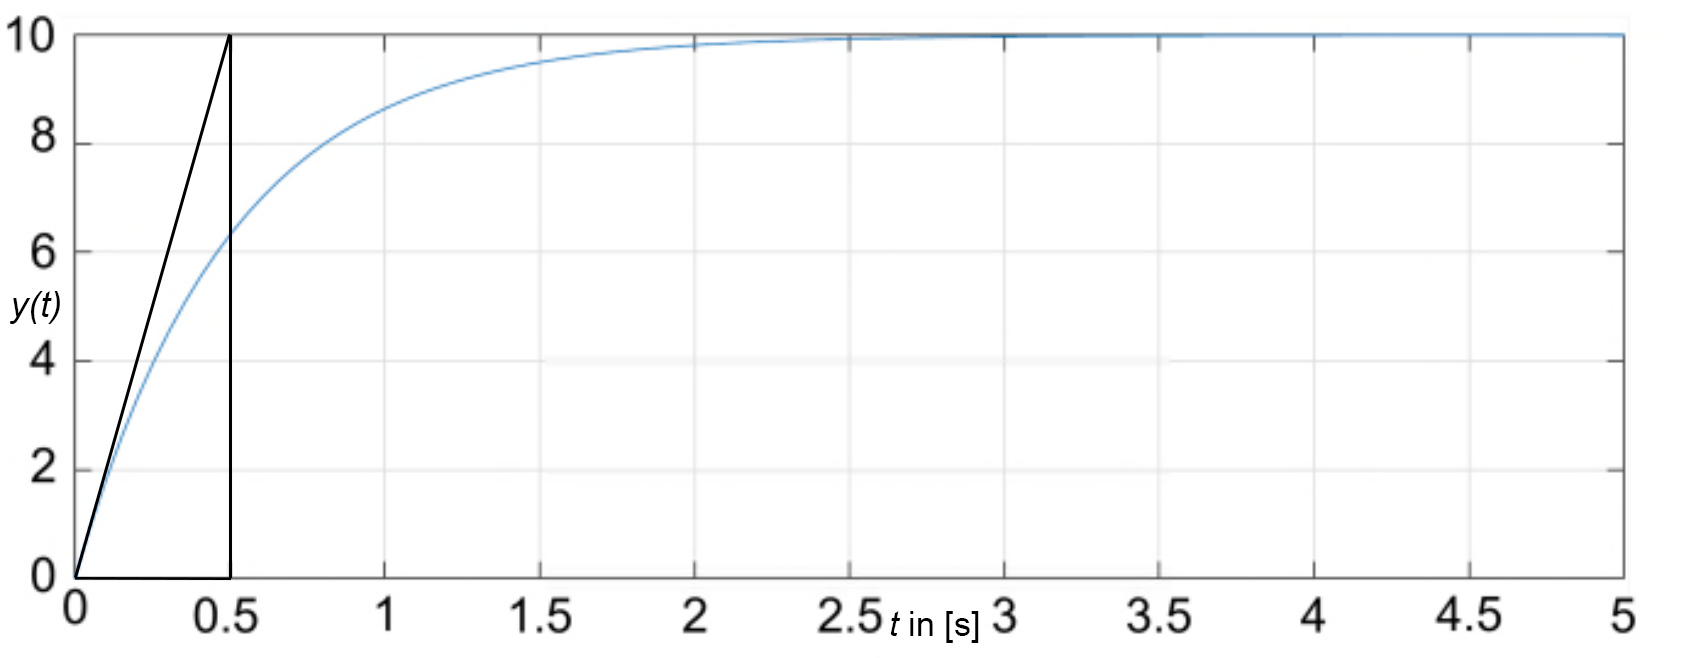
\includegraphics[width = 0.9 \textwidth]{./img/q1i1.png}
   \caption{Diagram to show step response of a first-order system.} 
   \label{fig:q1i1}
\end{figure}
Let us look at \ref{eq:q1i1}
\begin{equation}
    \frac{\dif y(t)}{\dif t} = ay(t) + b u(t)\label{eq:q1i1}
\end{equation}
Transforming to Laplace domain:
\begin{align}
    sY(s) - y(0) &= aY(s) + bU(s)
\end{align}
$y(0) = 0$:
\begin{align}
    Y(s)\left(s-a\right) &= bU(s)\\
    \frac{Y(s)}{U(s)} = \frac{b}{s-a}
\end{align}
For step input $U(s) = \frac{1}{s}$:
\begin{gather}
    Y(s) = \frac{b}{s(s-a)} = \frac{k_1}{s}+ \frac{k_2}{s-a}
\end{gather}
Solving partial fraction:
\begin{gather}
    k_1(s-a) + k_2 s = b\\
    s = 0 \rightarrow -ak_1 = b\\
    k_1 = -\frac{b}{a}\\
    s = a \rightarrow ak_2 = b\\
    k_2 = \frac{b}{a}\\
    Y(s) = \frac{b}{a(s-a)} - \frac{b}{as}\\
    Y(s) = \frac{b}{a}\left(\frac{1}{s-a}-\frac{1}{s}\right)
\end{gather}
Returning to time domain (using tables):
\begin{gather}
    y(t) = \frac{b}{a} \left(e^{at}-1\right) \label{eq:q1i2}\\
    \frac{\dif y(t)}{\dif t} = be^{at}\\
    \left. \frac{\dif y(t)}{\dif t} \right|_{t = 0} = b
\end{gather}
From Figure \ref{fig:q1i1}, we can see that the gradient at 0 is:
\begin{equation}
    b = \frac{10}{0.5} = 20
\end{equation}
Response settles at $y(t) = 10$, therefore:
\begin{align}
    e^{at} &= 0\\
    \therefore 10 &= \frac{20}{a}\left(-1\right)\\
    a &= -2
\end{align}
Hence:
\begin{align}
    y(t) = -10 \left(e^{-2t}-1\right)\\
    \frac{\dif y(t)}{\dif t} = -2y(t) + 10u(t)
\end{align}
\subsection{b}
\subsubsection{i}
\begin{align}
    \frac{\dif \omega(t)}{\dif t} &= -a\omega(t) + kv(t)\\
    s \theta(s) - \theta(0) &= -a \theta(s) + kV(s)\\
    s\theta(s) +a\theta (s) &= kV(s)\\
    \theta(s)\left(s+a\right) &= kV(s)\\
    \frac{\theta (s)}{V(s)} &= \frac{k}{s+a}\\
    \frac{\theta (s)}{V(s)} &= \frac{\frac{k}{a}}{\frac{s}{a}+1} = \frac{\gamma}{\tau s + 1}
\end{align}
Where $\gamma$ is the gain and $\tau$ is the time constant.
\subsubsection{ii}
\begin{figure}[H]
    \centering
    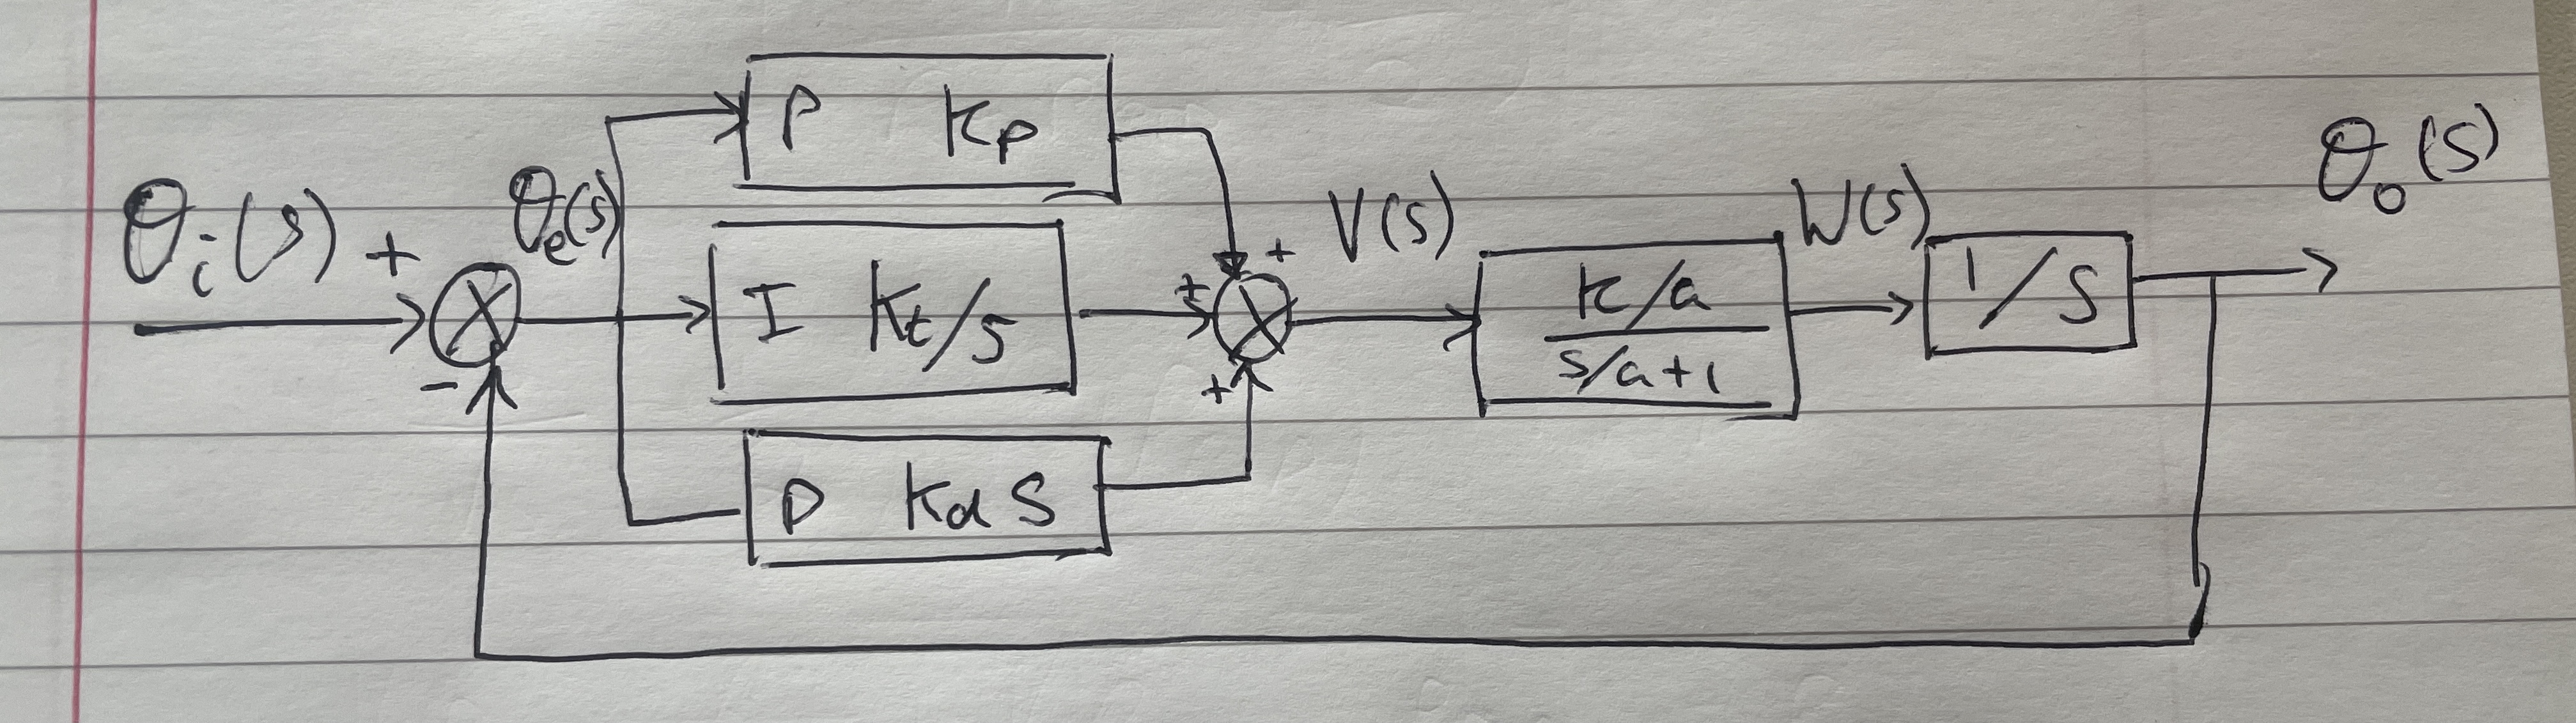
\includegraphics[height = 4cm]{./img/q1bii.jpg}
    \caption{Block diagram}
    \label{fig:q1bii}
\end{figure}
Computing loops:
\begin{align}
    F(s) &= \frac{\left(k_p + \frac{k_t}{s} + k_d s\right)\frac{\frac{k}{a}}{\frac{s}{a}+ 1}}{1 + \left(k_p + \frac{k_t}{s} + k_d s\right)\frac{\frac{k}{a}}{\frac{s}{a}+ 1}}\\
    F(s) &= \frac{k\left(s^2 k_d + sk_p + k_t\right)}{s\left(s+a\right)+k\left(s^2 k_d + sk_p + k_t\right)}
\end{align}
\subsection{c}
\subsubsection{i}
Let us start by performing a block diagram reduction, to simplify finding the transfer function of the system.
\begin{figure}[H]
    \centering
    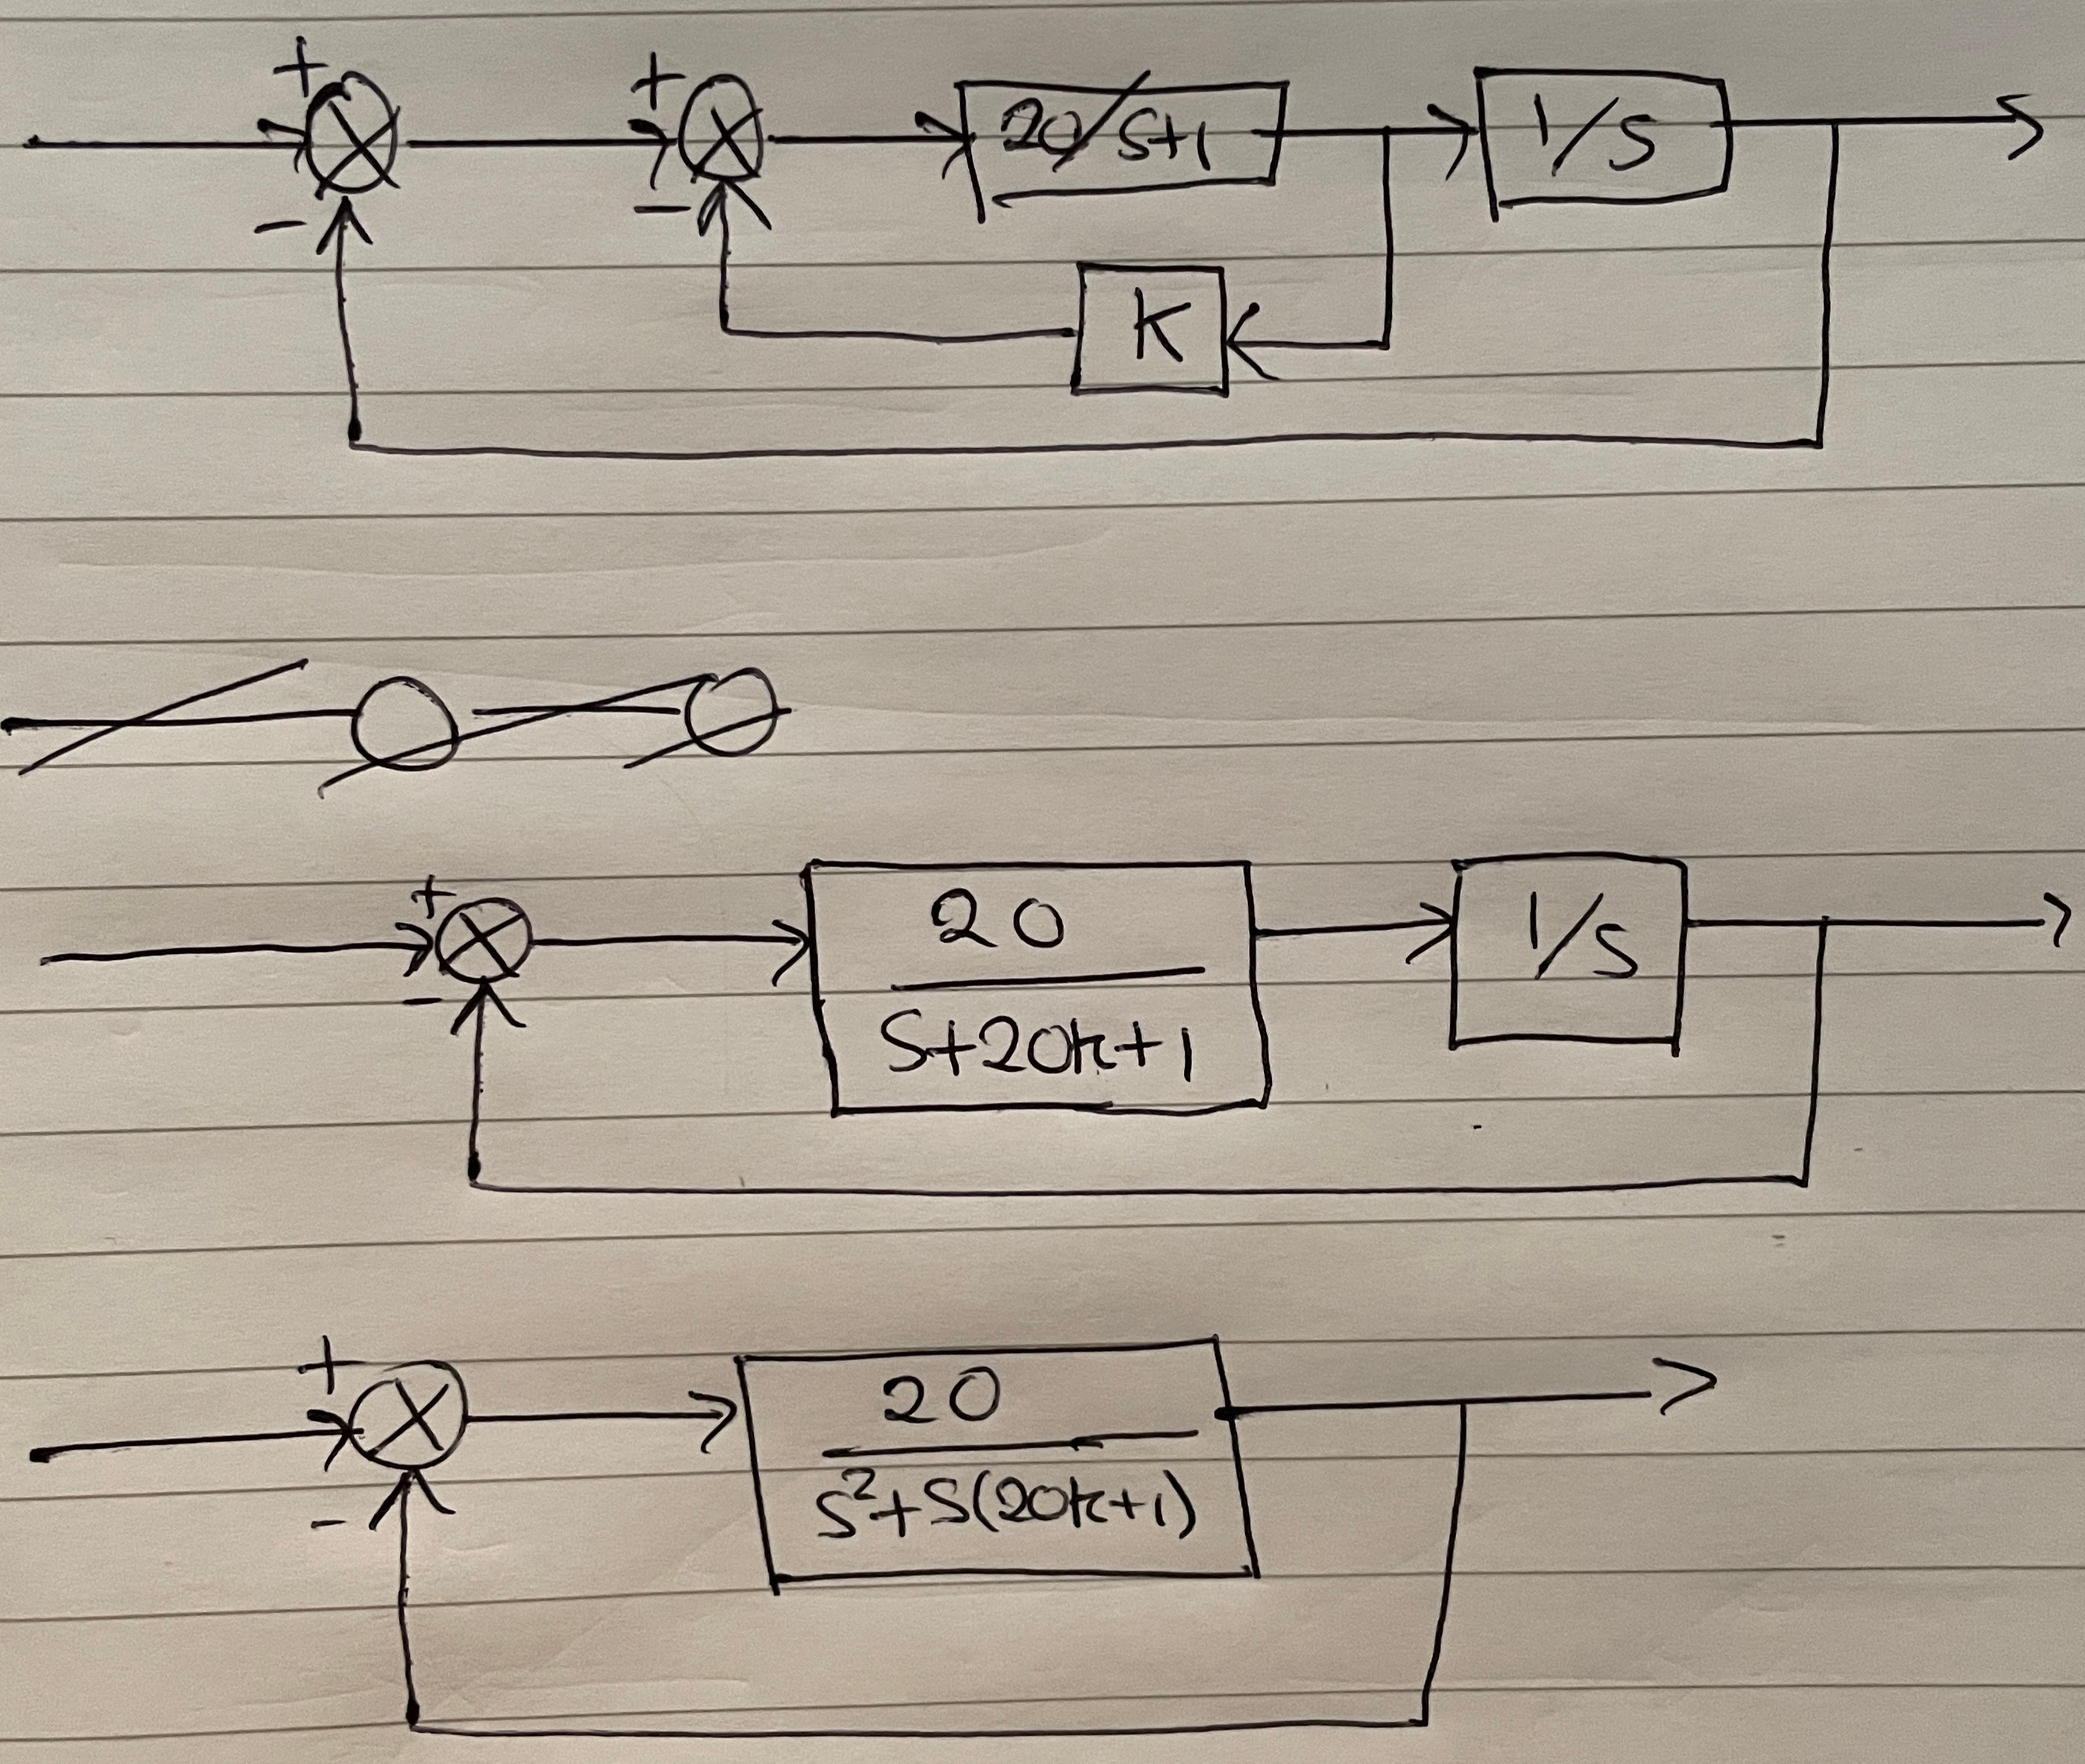
\includegraphics[height = 10cm]{./img/q1ci.jpg}
    \caption{Reduction of block diagram}
\end{figure}
Reduction of first loop:
\begin{align}
    G_1(s) &= \frac{\frac{20}{s+1}}{1 + \frac{20k}{s+1}}\\
    G_1(s) &= \frac{20}{s + 20k +1}
\end{align}
Simplifying second loop:
\begin{align}
    G_2(s) &= \frac{1}{s}\cdot\frac{20}{s+20k+1}\\
    G_2(s) &= \frac{20}{s^2 + s(20k+1)}
\end{align}
Final transfer function:
\begin{align}
    F(s) &= \frac{\frac{20}{s^2 + s(20k+1)}}{1 + \frac{20}{s^2 + s(20k+1)}}\\
    F(s) &= \frac{20}{s^2 + s(20k+1) + 20}
\end{align}
We know that the standard form of a second order transfer function is: 
\begin{align}
    F(s) &= \gamma\frac{\omega_n^2}{s^2 + 2\zeta \omega_n s +  \omega_n^2}
\end{align}
Comparing coefficients:
\begin{align}
    20k+ 1 &= 2\zeta \omega_n
\end{align}
Where $\omega_n = \sqrt{20}$ and $\zeta = 0.4$. Therefore:
\begin{align}
    20 k + 1 &= 2 (0.4)\sqrt{20}\\
    k &= \frac{-5+8\sqrt{5}}{100} = 0.129 \textrm{ (3sf)}
\end{align}
\subsubsection{ii}
\begin{figure}[H]
    \centering
    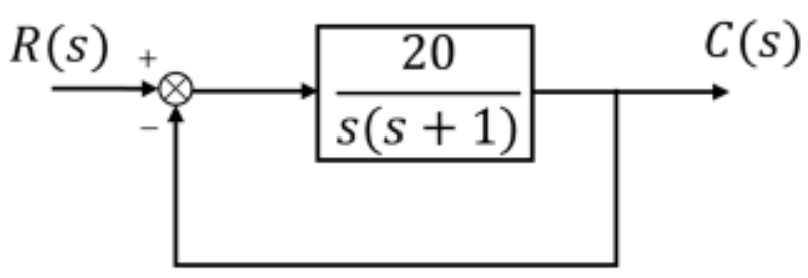
\includegraphics[height = 3cm]{./img/q1cii1.png}
    \caption{Block diagram}
    \label{fig:q1cii1}
\end{figure}
Transfer function of Figure \ref{fig:q1cii1}:
\begin{align}
    F(s) &= \frac{\frac{20}{s(s+1)}}{1 + \frac{20}{s(s+1)}}\\
    F(s) &= \frac{20}{s^2 + s + 20 }
\end{align}
We know that the standard form of a second order transfer function is: 
\begin{align}
    F(s) &= \gamma\frac{\omega_n^2}{s^2 + 2\zeta \omega_n s +  \omega_n^2}
\end{align}
Comparing coefficients:
\begin{align}
    \omega_n &= \sqrt{20}\\
    1&= 2\zeta \sqrt{20}\\
    \zeta &= \frac{\sqrt{5}}{20}
\end{align}
Therefore, the overshoot can be calculated as:
\begin{align}
    A &= e^{\frac{-\zeta \pi}{\sqrt{1-\zeta^2}}}\\
    A &= e^{\frac{-\frac{\sqrt{5}}{20} \pi}{\sqrt{1-\left(\frac{\sqrt{5}}{20}\right)^2}}}\\
    A &= 0.702 \textrm{ (3sf)}
\end{align}
Rise time:
\begin{align}
    t_r &= \frac{1}{\omega_n \sqrt{1- \zeta^2}} \left(\pi - \arctan\left(\frac{\sqrt{1-\zeta^2}}{\zeta}\right)\right)\\
    t_r &= \frac{1}{\sqrt{20} \sqrt{1- \left(\frac{\sqrt{5}}{20}\right)^2}} \left(\pi - \arctan\left(\frac{\sqrt{1-\left(\frac{\sqrt{5}}{20}\right)^2}}{\frac{\sqrt{5}}{20}}\right)\right)\\
    t_r &= \SI{0.379}{\second} \textrm{ (3sf)}
\end{align}
Peak time:
\begin{align}
    t_p &= \frac{\pi}{\omega_n \sqrt{1- \zeta^2}}\\
    t_p &= \frac{\pi}{\sqrt{20} \sqrt{1- \left(\frac{\sqrt{5}}{20}\right)^2}}\\
    t_p &= \SI{0.707}{\second} \textrm{ (3sf)}
\end{align}
Settling time (5\%):
\begin{align}
    e^{-\zeta\omega_n t_s} &= 0.05\\
    t_s &= \frac{-\ln\left(0.05\right)}{\frac{\sqrt{5}}{20} \sqrt{20}}\\
    t_s &= \SI{5.99}{\second} \textrm{ (3sf)}
\end{align}
Steady state value:
\begin{align}
    C(t_s) &= 1 - \frac{1}{\sqrt{1-\zeta^2}}e^{-\zeta \omega_n t_s}\sin\left(\omega_n \sqrt{1-\zeta^2}t_s + \arccos\left(\zeta\right)\right)\\
    C(t_s) &= 1 - \frac{1}{\sqrt{1-\left(\frac{\sqrt{5}}{20}\right)^2}}e^{-\dfrac{5.99\sqrt{20}\sqrt{5}}{20}}\sin \left(5.99\sqrt{20} \sqrt{1-\left(\frac{\sqrt{5}}{20}\right)^2}  + \arccos\left(\frac{\sqrt{5}}{20}\right)\right)\\
    C(t_s) &= 0.990 \textrm{ (3sf)}
\end{align}
Using the information from part Q1ci, the values of the constants from the other block diagram were inputted into the above diagrams and are shown in \ref{tab:q1cii1}
\begin{table}[H]
    \centering
    \begin{tabular}{lll}
        \toprule
        & \multicolumn{2}{c}{Transfer function}\\
        \cmidrule{2-3}
        & $F(s) = \dfrac{20}{s^2 + s + 20 }$ & $F(s) = \dfrac{20}{s^2 + s(20k+1) + 20}$\\
        Variable (3sf) & No feedback & With feedback\\
        \midrule
        Overshoot $A$ & 0.702 & 0.254 \\
        Rise time $t_r$ (\si{second}) & 0.379 & 0.484 \\
        Peak time $t_p$ (\si{second})& 0.707 & 0.766\\
        Settling time $t_s$ (5\%) (\si{\second}) & 5.99 & 1.68\\
        Steady state value & 0.990 & 0.990\\
        \bottomrule
    \end{tabular}
    \caption{Table to show values of overshoot, rise time, peak time, settling time and steady state value.}
    \label{tab:q1cii1}
\end{table}
\subsection{d}
\subsubsection{i}
Looking at time domain:
\begin{align}
    v_i(t) = v_o(t) + v_p(t)
\end{align}
Where $v_p$ represents the voltage across the parallel section. Looking at $v_o$:
\begin{align}
    v_o(t) = R_1 i(t) + \dfrac{1}{C_1}\int \left(i(t)\right)\dif t
\end{align}
Converting to frequency domain:
\begin{align}
    V_o(s) &= I(s) R_1 + \dfrac{I(s)}{sC_1}\\
    V_o(s) &= I(s) \left(R_1 + \dfrac{1}{sC_1}\right) \label{eq:q1di1}
\end{align}
Looking at $v_p$, we know that the voltage is equal across the two branches, let us instead look at the current:
\begin{align}
    i(t) &= i_{R_2}(t) + i_{C_2}(t)\\
    i(t) &= \frac{v_p(t)}{R_2} + C_2 \dfrac{\dif v_p(t)}{\dif t}
\end{align}
Converting to frequency domain:
\begin{align}
    I(s) &= \frac{V_p(s)}{R_2} + sC_2V_p(s)\\
    I(s) &= V_p(s) \left(\frac{1}{R_2} + sC_2\right)\\
    V_p(s) &= \frac{I(s)}{\frac{1}{R_2}+sC_2} \label{eq:q1di2}
\end{align}
Using \ref{eq:q1di1} and \ref{eq:q1di2}:
\begin{align}
    V_i(s) &= V_o(s) + V_p(s)\\
    V_i(s) &= I(s) \left(R_1 + \dfrac{1}{sC_1}\right) + \frac{I(s)}{\frac{1}{R_2}+sC_2}\\
    V_i(s) &= I(s) \left(R_1 + \dfrac{1}{sC_1} + \dfrac{1}{\frac{1}{R_2} + sC_2}\right) \label{eq:q1di3}
\end{align}
Using \ref{eq:q1di1} and \ref{eq:q1di3}:
\begin{align}
    \dfrac{V_o(s)}{V_i(s)} &= \dfrac{I(s) \left(R_1 + \dfrac{1}{sC_1}\right)}{I(s) \left(R_1 + \dfrac{1}{sC_1} + \dfrac{1}{\frac{1}{R_2} + sC_2}\right)}\\
    \dfrac{V_o(s)}{V_i(s)} &= \dfrac{R_1 + \dfrac{1}{sC_1}}{R_1 + \dfrac{1}{sC_1} + \dfrac{1}{\frac{1}{R_2} + sC_2}}\\
    \dfrac{V_o(s)}{V_i(s)} &= \frac{\left(sR_1 C_1 + 1 \right)\left(sR_2C_2 + 1\right)}{sR_1 C_1 \left(sR_2C_2 + 1\right) + sR_2 C_2 + 1 + sC_1 R_2}\\
    \dfrac{V_o(s)}{V_i(s)} &= \frac{\left(sR_1 C_1 + 1 \right)\left(sR_2C_2 + 1\right)}{\left(sR_1 C_1 + 1 \right)\left(sR_2C_2 + 1\right) + sC_1 R_2 }
\end{align}
\subsubsection{ii}
We can derive a mechanical system from an electrical system using analogues. We can represent a resistor with a damper and a capacitor with a spring. Drawing, the new mechanical system we get:
\begin{figure}[H]
    \centering
    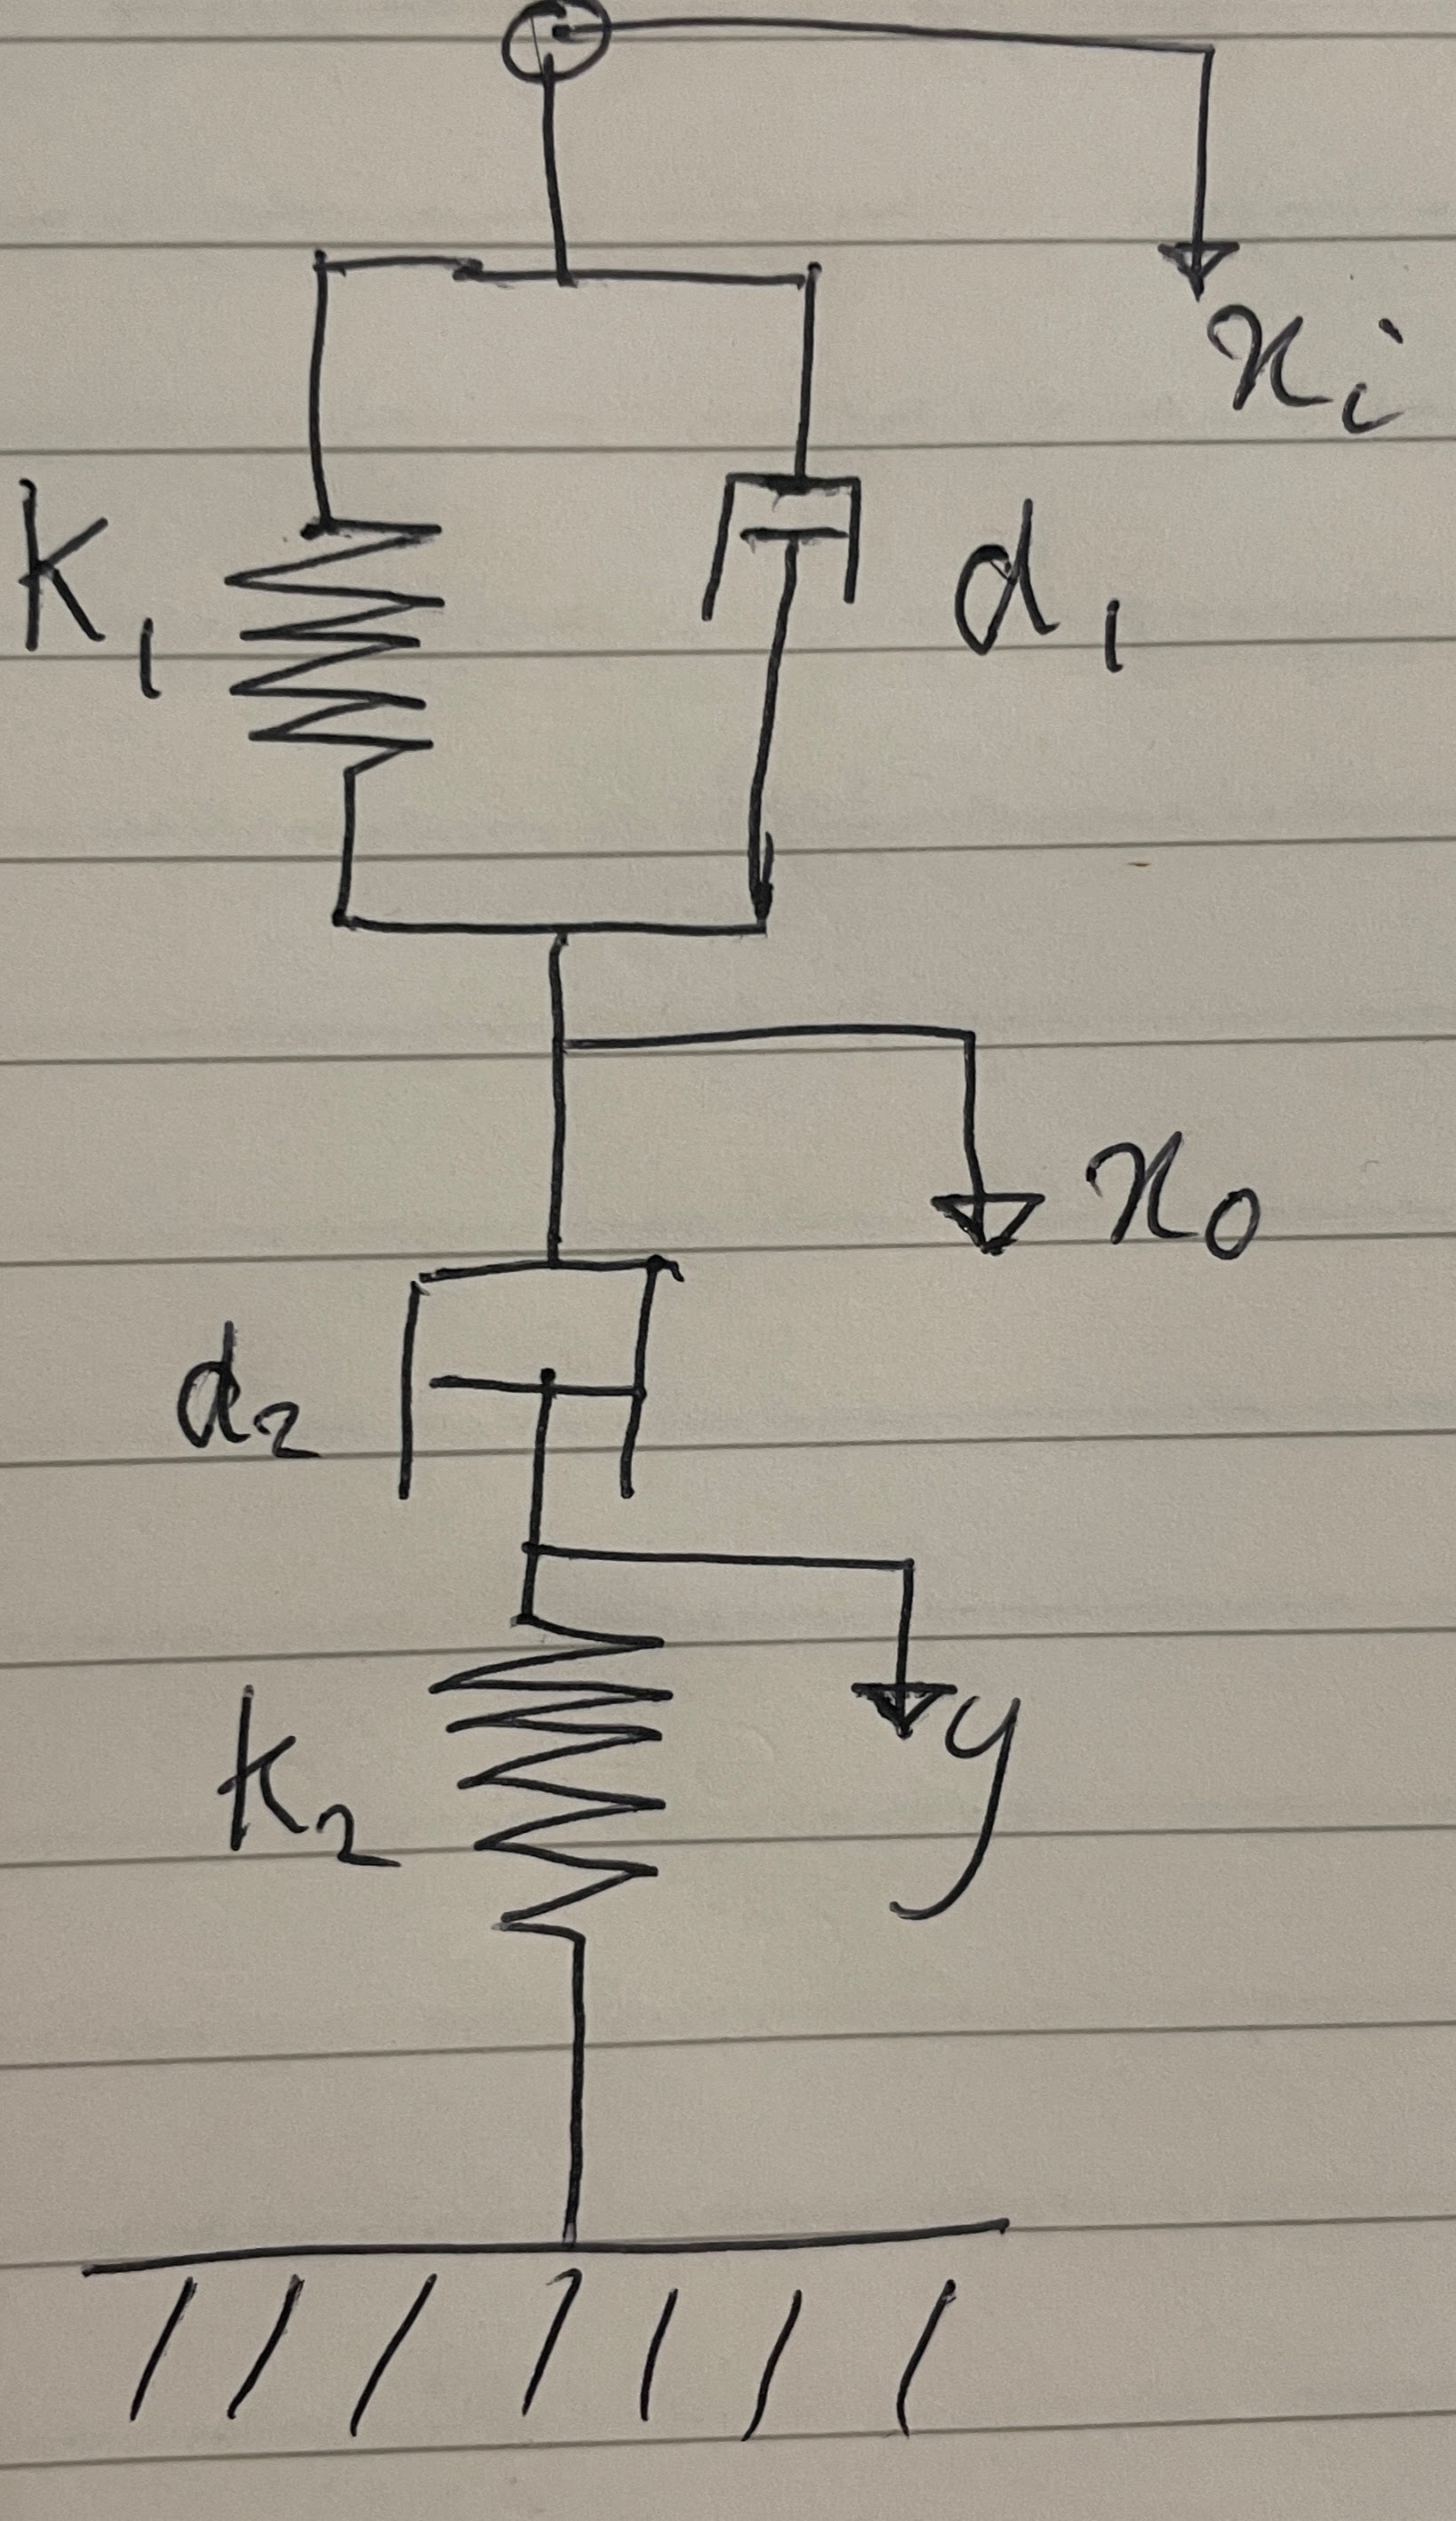
\includegraphics[height = 8cm]{./img/q1dii1.jpg}
    \caption{Mechanical representation of system.}
    \label{fig:q1dii1}
\end{figure}
We can now analyse the mechanical system by looking at the displacement at each point:
\begin{align}
    d_1 (x_i - x_o) + k_1 (x_i - x_o) &= d_2 (x_0 - y)\\
    d_2 (x_o - y) &= k_2 y
\end{align}
Converting to frequency domain and assuming the following boundary conditions:
\begin{gather}
    x_i(0) = 0, \; x_o(0) = 0, \; y(0) = 0
\end{gather}
\begin{align}
    d_1 \left[sX_i(s) - sX_o(s)\right] + k_1 \left[X_i(s) - X_o(s)\right] &= d_2 \left[sX_o(s) - sY(s)\right]\\
    d_2\left[sX_o(s)-sY(s)\right] &= k_2Y(s)
\end{align}
Rearranging for $Y(s)$ and substituting:
\begin{align}
    Y(s) &= \dfrac{d_2sX_o(s)}{d_2s +k_2}\\
    d_1 \left[sX_i(s) - sX_o(s)\right] + k_1 \left[X_i(s) - X_o(s)\right] &= d_2 \left[sX_o(s) - s\dfrac{d_2sX_o(s)}{d_2s +k_2}\right]
\end{align}
Simplifying and factorising:
\begin{align}
    X_i(s)\left(d_1 s + k_1\right) &= X_o(s) \left(d_1 s + k_1 + d_2 s - \dfrac{d_2^2 s^2}{d_2s + k_2}\right)
\end{align}
Dividing to find $\dfrac{X_o(s)}{X_i(s)}$:
\begin{align}
    \dfrac{X_o(s)}{X_i(s)} &= \dfrac{d_1 s + k_1}{d_1 s + k_1 + d_2 s - \dfrac{d_2^2 s^2}{d_2s + k_2}}
\end{align}
Factorising:
\begin{align}
    \dfrac{X_o(s)}{X_i(s)} &= \dfrac{\left(\frac{d_1s}{k_1} + 1\right)\left(\frac{d_2s}{k_2} + 1\right)}{\left(\frac{d_1s}{k_1} + 1\right)\left(\frac{d_2 s}{k_2}+1\right) + \frac{d_2s}{k_1}}
\end{align}
\section{Question 2}
To measure gas flow, we will be looking at the changes in current delivered to a hot wire anemometer, specifically a constant temperature anemometer. They are small, thin wires suspended in the flow, heated by a current. A circuit diagram is shown in Figure \ref{fig:q2i1}
\begin{figure}[H]
    \centering
    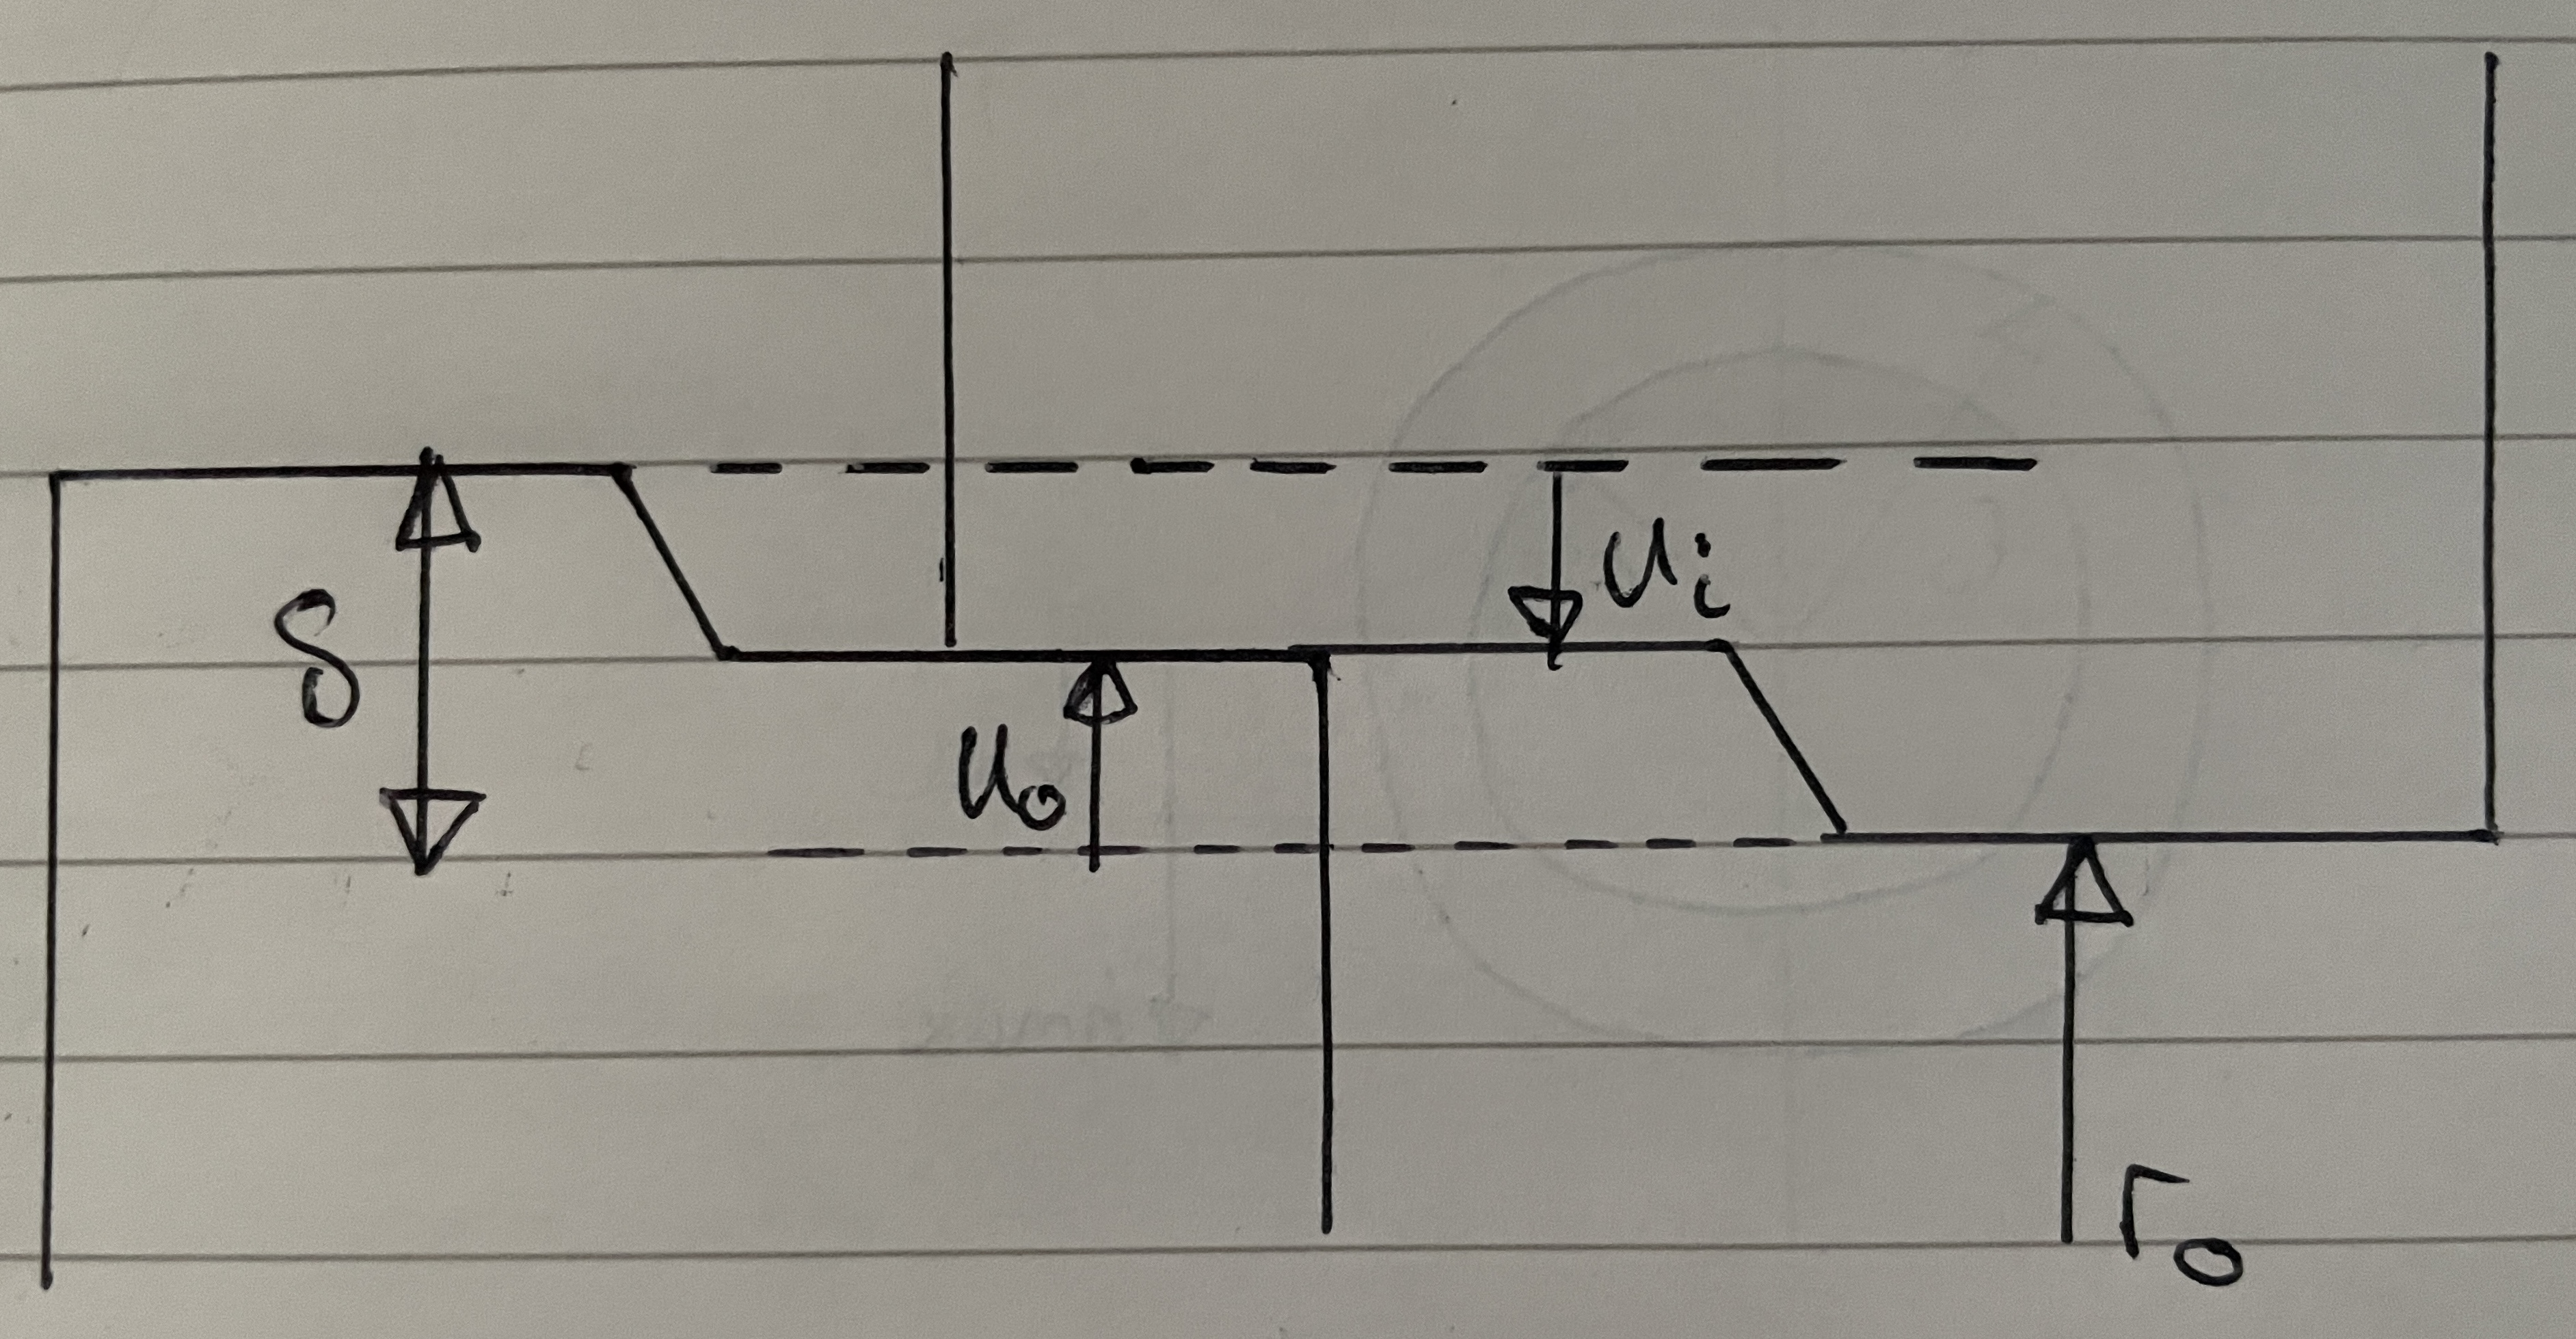
\includegraphics[height = 5cm]{./img/q2i1.jpg}
    \caption{Diagram to show basic circuit for a hot wire anemometer working in constant temperature mode.} 
    \label{fig:q2i1}
 \end{figure}
This Wheatstone bridge keeps the anemometer a constant temperature, which is important to measure the flow. We know that the resistance of a wire is proportional to its temperature and if we can maintain the temperature at a certain value, then we will be able to maintain its resistance. We can connect the anemometer to a Wheatstone bridge. Initially our bridge is balanced and as fluid flows past our wire, there is heat transfer at a constant rate. As the velocity of the fluid changes, the rate of thermal heat transfer also changes. In the case that flow rate increases, the increased heat transfer causes the temperature of the wire to decrease, decreasing its resistance. This causes the bridge to become unbalanced. From Figure \ref{fig:q2i1}, an $e^+$ signal is sent to the op-amp. After amplification, the bridge voltage is increased and current flow through the wire is increased. An increase in current, leads to an increase in temperature and resistance, balancing the bridge once more \cite{b1}.

Use of a hot wire anemometer is justified as they are small sensors (millimetre scale) and can be used in high temperature situations. Their range of measurement is very high and suitable for this use case. The TSI model 1222 can be used in fluids up to \SI{300}{\celsius} \cite{b3}. They have high frequency response but are fragile, relatively expensive and require clean gas flows to prevent damage \cite{b3}. For an accurate measurement of the flow in the pipe, we should place our sensor near the centre of the cross-section as the flow would be less affected by boundary layer effects.

To derive the flow velocity as a function of current, we need to look at three equations: power equilibrium conditions (\ref{eq:q2i1}), wire resistance as a function of temperature (\ref{eq:q2i2}) and King's law (\ref{eq:q2i3}). 
\begin{align}
    I^2 R_w &= h A_w \left(T_w - T_f\right)\label{eq:q2i1}\\
    R_w &= R_{ref} \left[1 + \alpha\left(T_w - T_{ref}\right)\right] \label{eq:q2i2}\\
    h &= A + B v_f^c \label{eq:q2i3}
\end{align}
Where $I$ is current, $R_{ref}$, $T_{ref}$, calibration resistance and temperature, $T_w$, $T_f$, wire and fluid temperatures, $A_w$ wire projected surface area, $\alpha$, thermal coefficient of resistance, $h$ heat transfer coefficient of wire, $A$, $B$, $c$ are calibration constants and $v_f$ is the gas flow \cite{b2}. Substituting and rearranging:
\begin{align}
    v_f &= \left[\frac{I^2 R_{ref}\left[1 + \alpha \left(T_w - T_{ref}\right)\right]}{BA_w \left(T_w - T_f\right)}-\frac{A}{B}\right]^{\frac{1}{c}} \label{eq:q2i}\\
    v_f &= f(I, T_f)
\end{align}
\section{Question 3}
\subsection{a}
\begin{figure}[H]
    \centering
    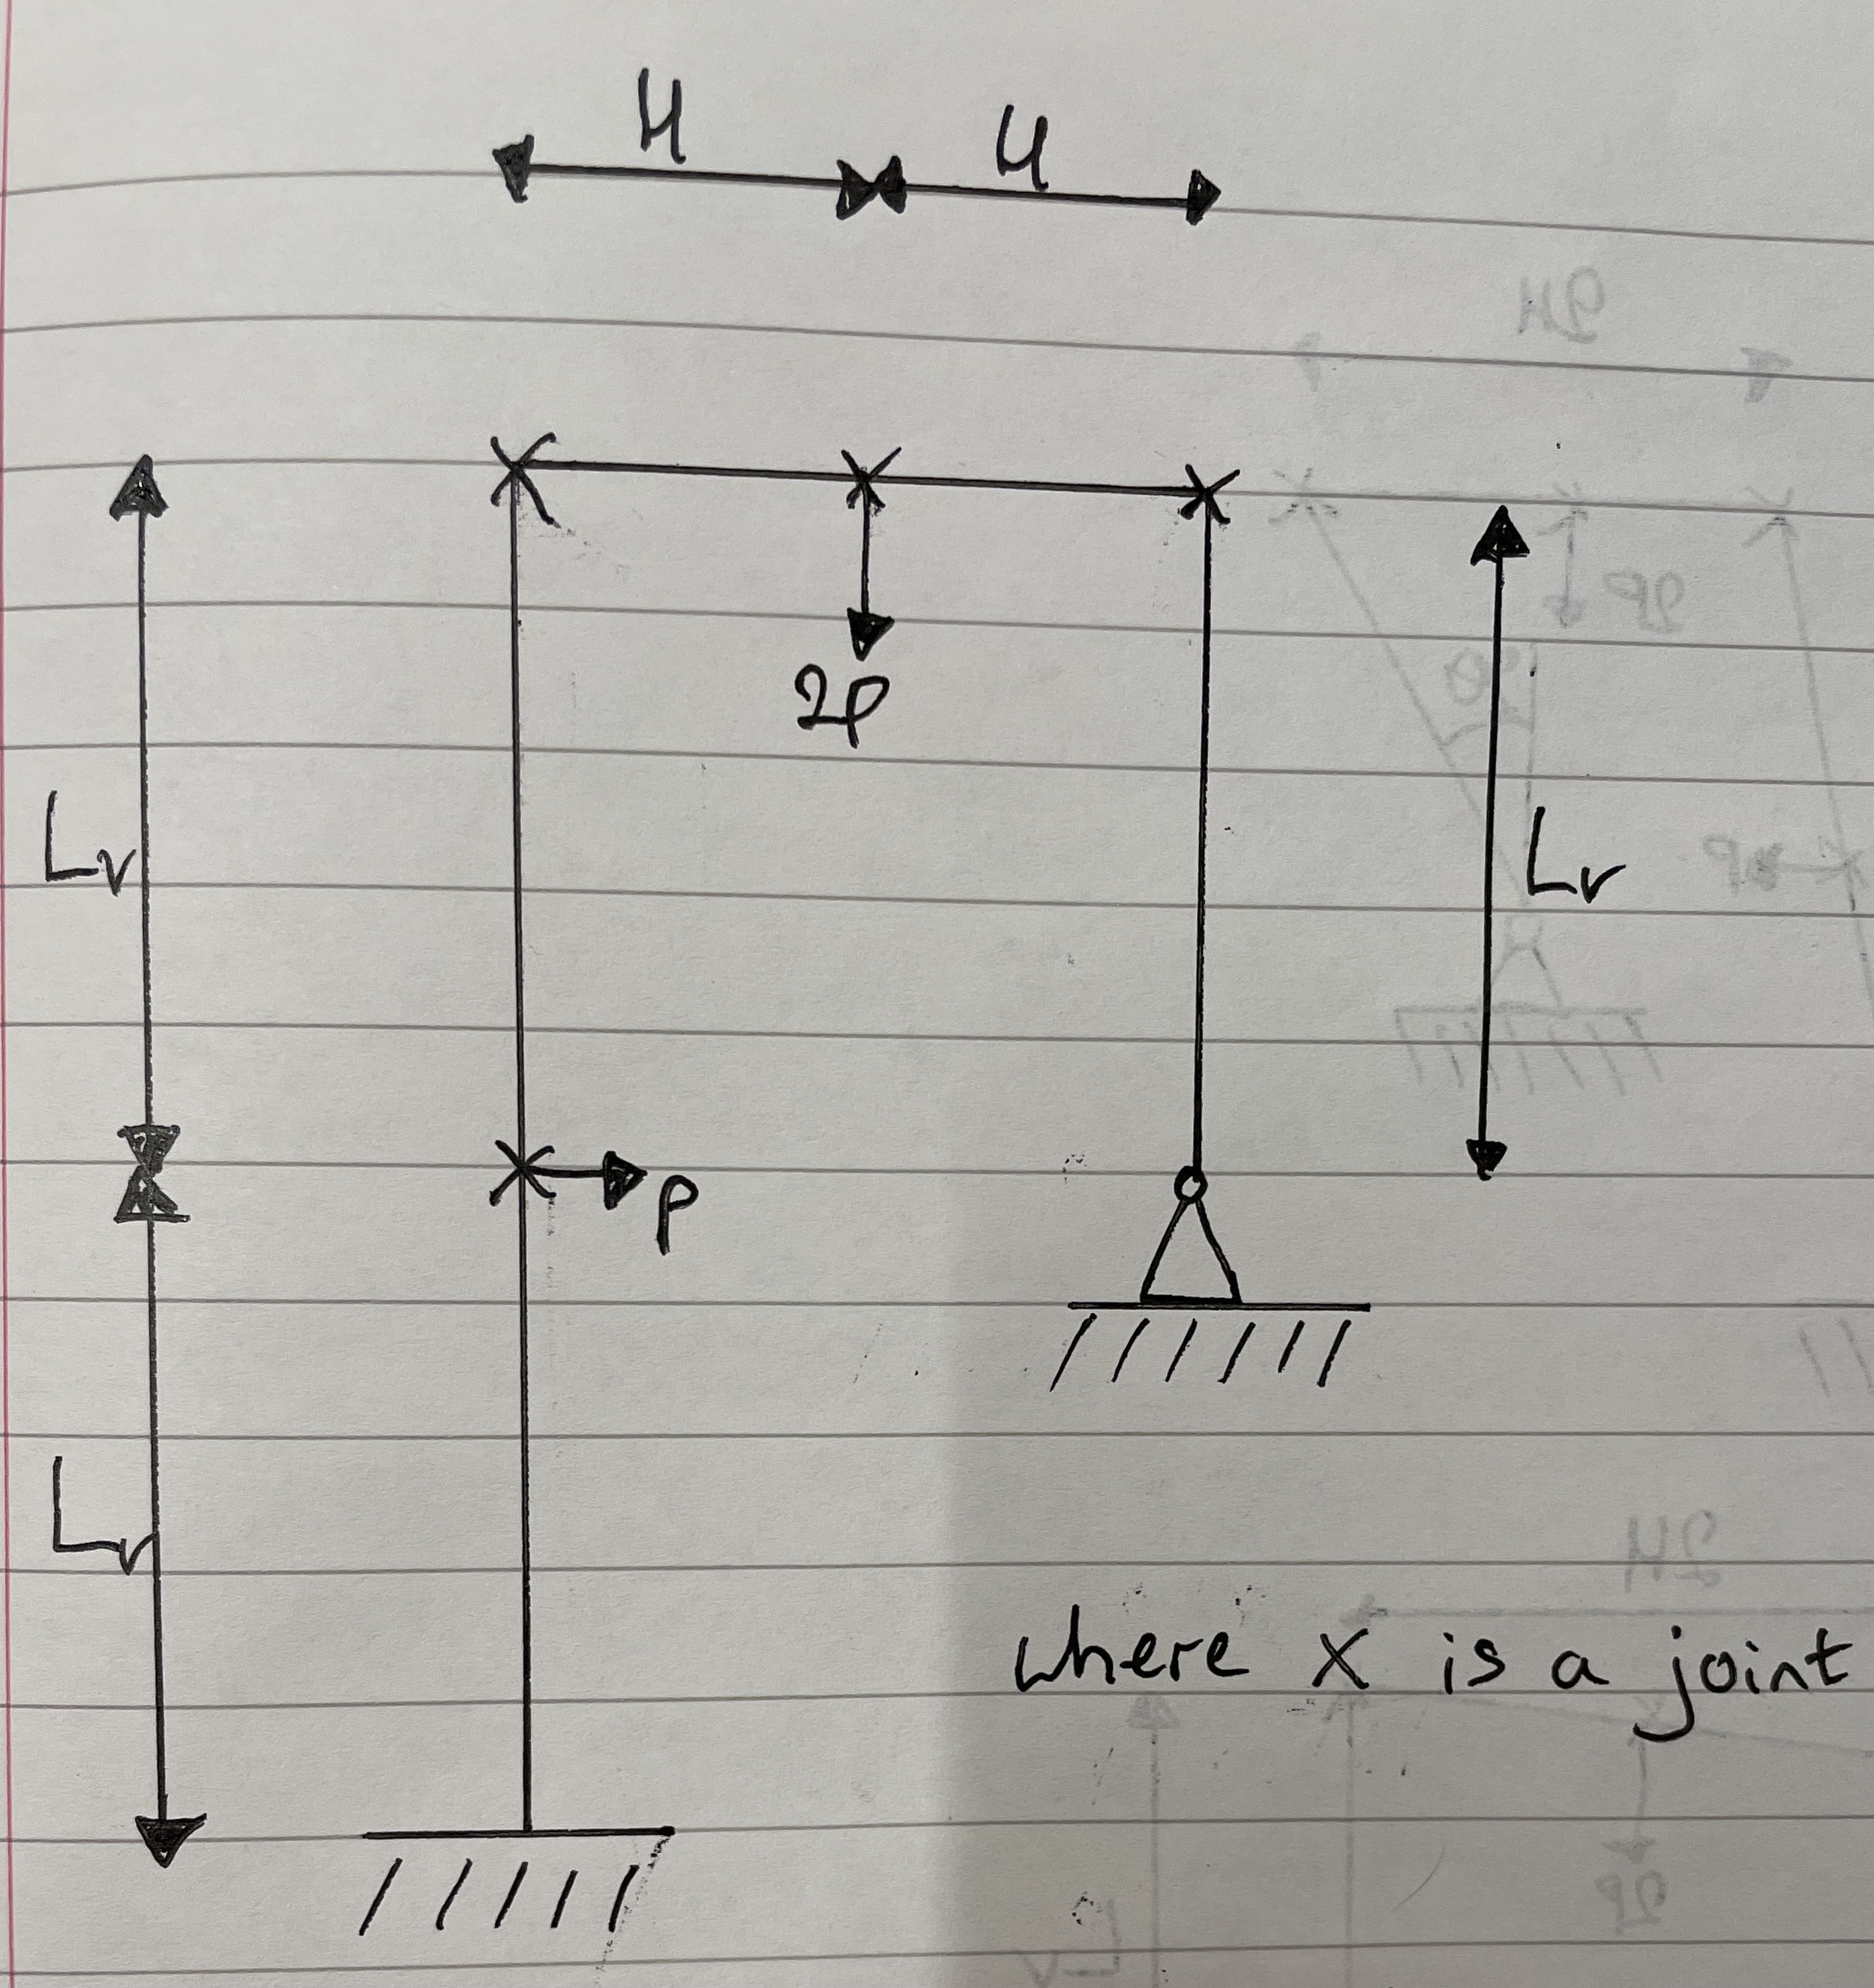
\includegraphics[height = 5cm]{./img/q3i1.jpg}
    \caption{Diagram to show physical seismic mass accelerometer.} 
    \label{fig:q3i1}
\end{figure}
\begin{figure}[H]
    \centering
    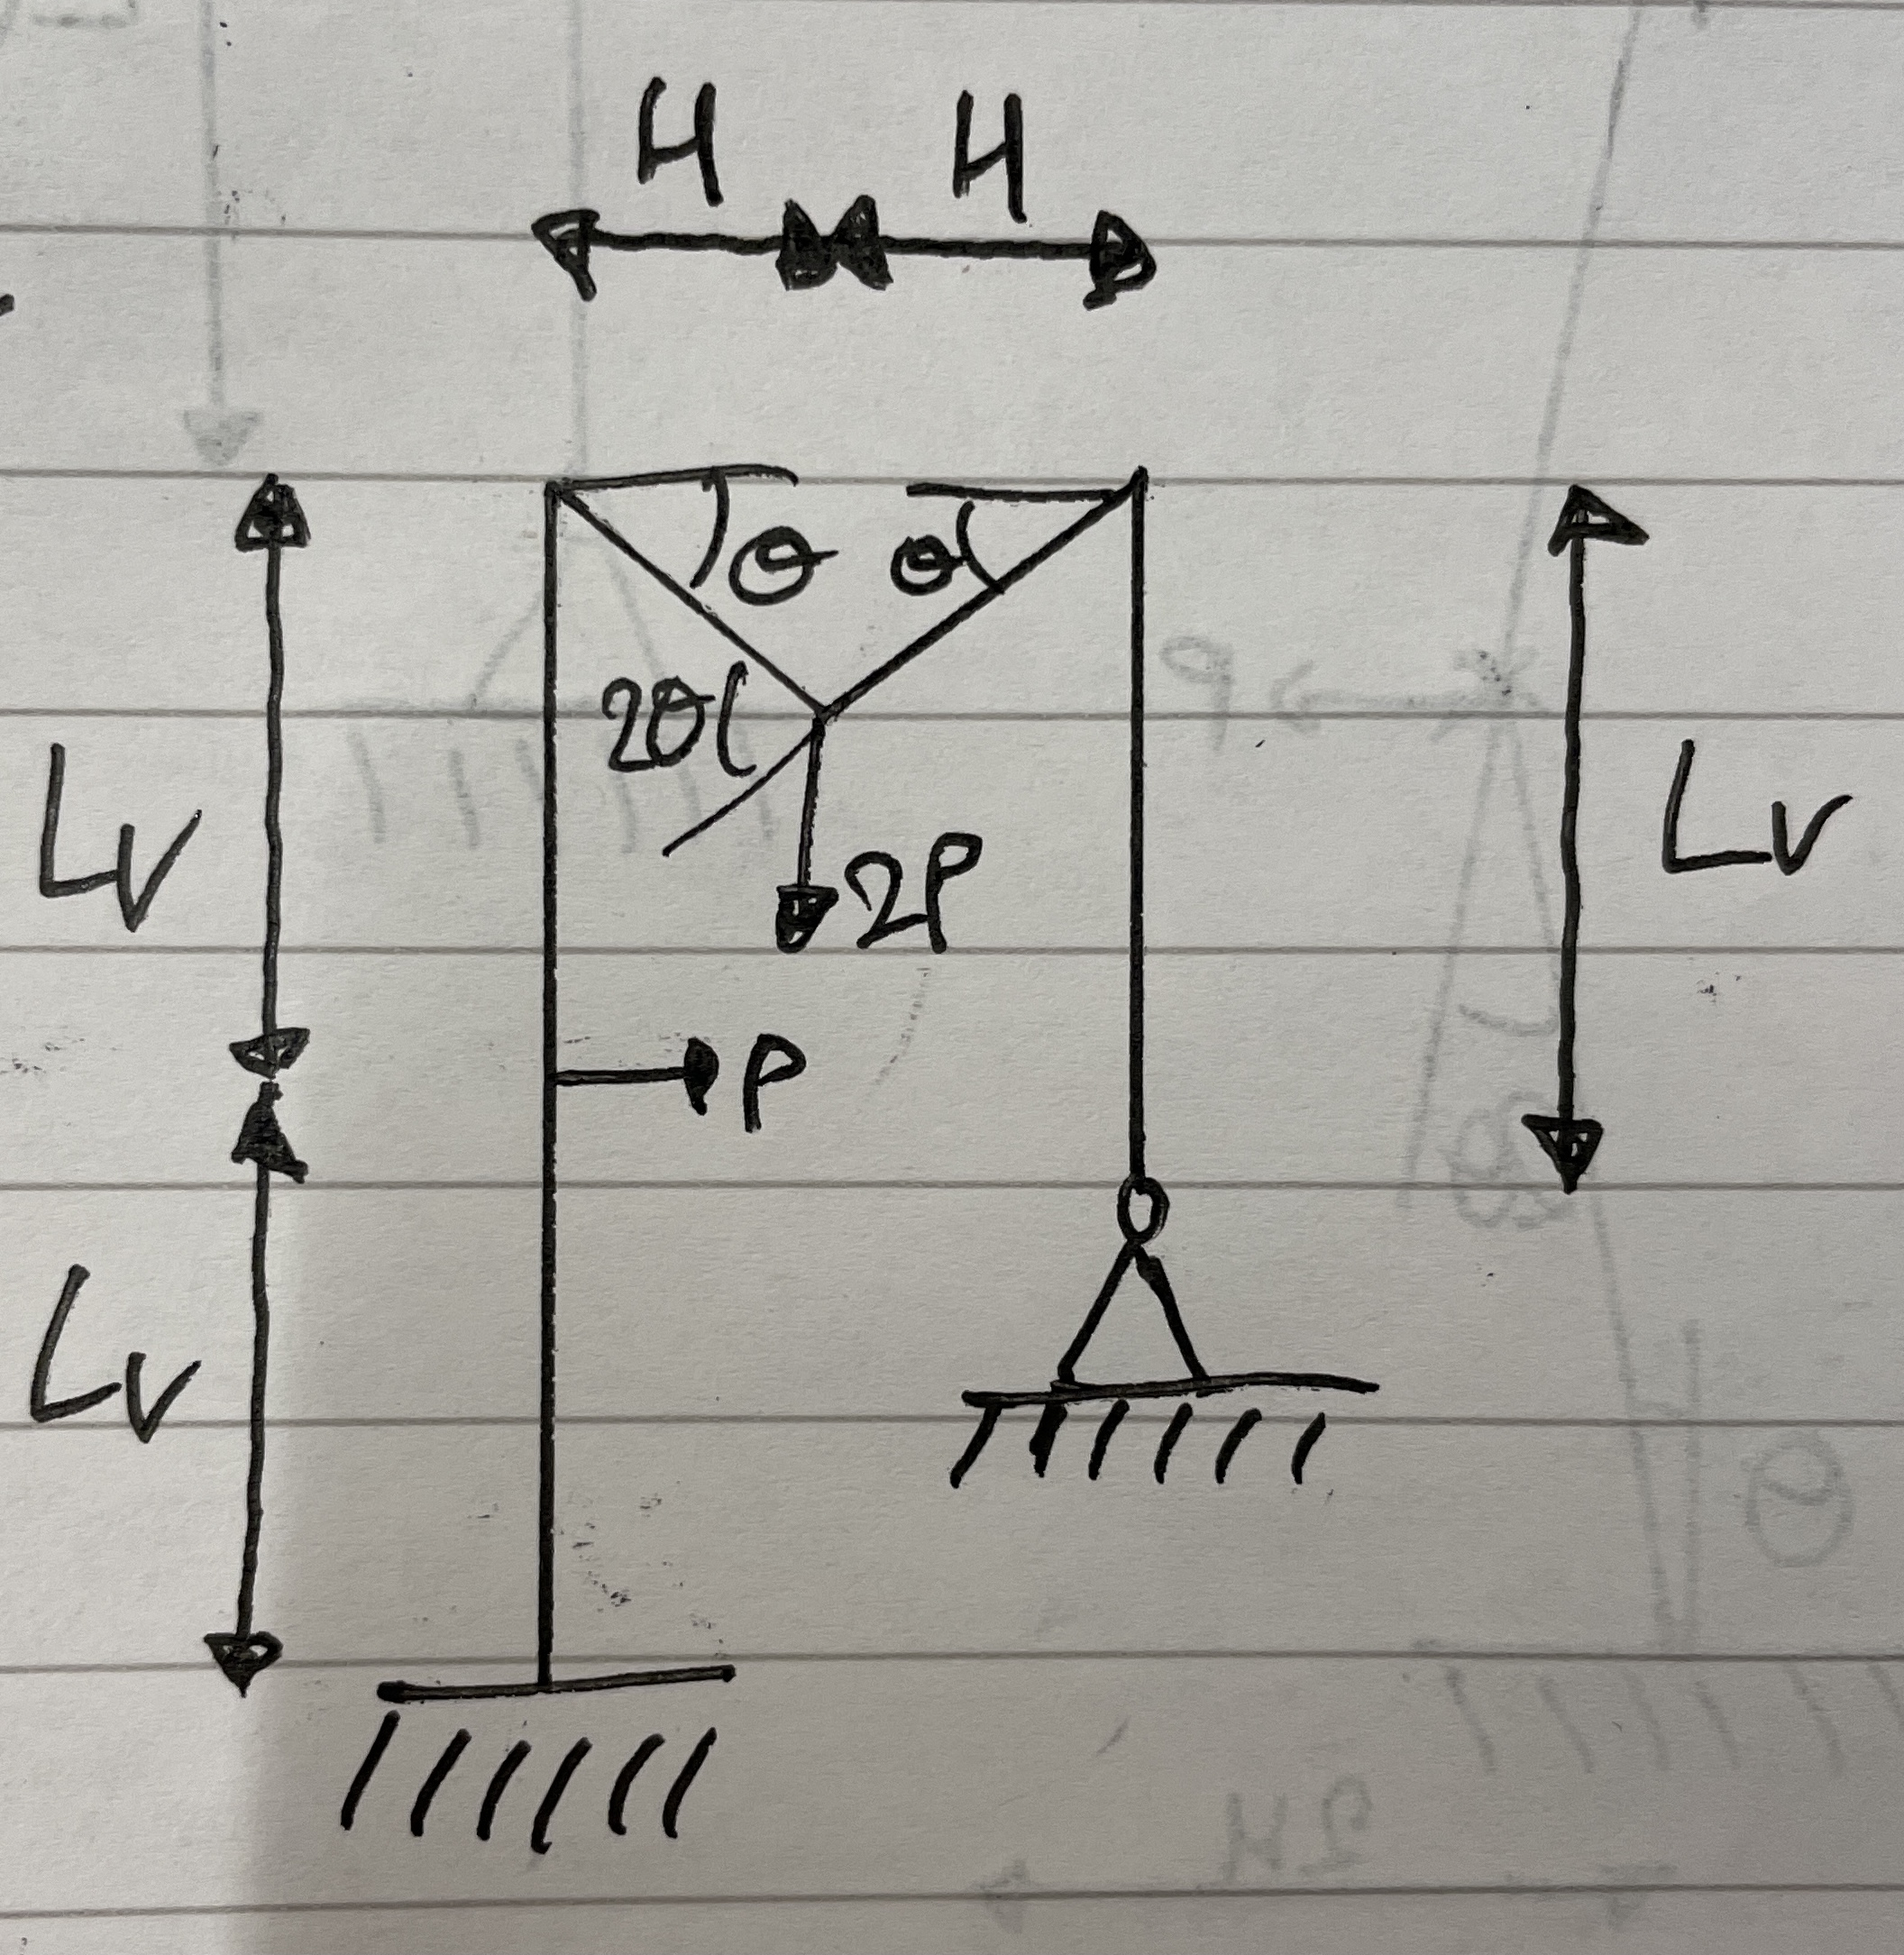
\includegraphics[height = 5cm]{./img/q3i2.jpg}
    \caption{Diagram to show arrangement of circuit.} 
    \label{fig:q3i2}
\end{figure}
The seismic mass accelerometer is attached to the outside of the pipe and composes of a mass suspended by a spring, with a damper. A wiper is positioned on a potentiometer such that when the seismic mass moves, it moves proportionally. This allows the resistance of the potentiometer to vary proportionally to the displacement of the mass. At the initial position, we can take the convention that the wiper blade sits in the middle of the potentiometer ($\frac{L}{2}$). From Newton's second law and Hooke's law, we know that:
\begin{align}
    F &= ma\\
    F &= kx\\
    a &= \frac{kx}{m} \label{eq:q3i5}
\end{align}
From Figure \ref{fig:q3i1} and \ref{fig:q3i2}, we can split our potentiometer such that $R_p = R_2 + R_3$. Hence:
\begin{align}
    R_2 &= \frac{R_p x}{L}\label{eq:q3i1}\\
    R_3 &= \frac{R_p (L-x)}{L}\label{eq:q3i2}
\end{align} 
Using Ohm's law:
\begin{align}
    V_o = \frac{\frac{R_2 R_1}{R_2 + R_1}}{R_3 + \frac{R_2 R_1}{R_2 + R_1}}V_s
\end{align}
Simplifying:
\begin{align}
    V_o= \frac{R_1 R_2}{R_3\left(R_1 + R_2\right) + R_1 R_2}V_s \label{eq:q3i3}
\end{align}
Substituting \ref{eq:q3i1} and \ref{eq:q3i2} into \ref{eq:q3i3}:
\begin{align}
    V_o= \frac{R_1\frac{R_p x}{L}}{\frac{R_p (L-x)}{L}\left(R_1 + \frac{R_p x}{L}\right) + R_1 \frac{R_p x}{L}}V_s 
\end{align}
Simplifying:
\begin{align}
    V_o = \frac{LR_1 x}{L^2 R_1 + LxR_p - x^2 R_p}V_s
\end{align}
Assuming that $R_1 >> R_p$, we can neglect our $R_p$ terms, leaving us with:
\begin{align}
    V_o &= \frac{LR_1 x}{L^2 R_1}V_s\\
    V_o &= \frac{x}{L}V_s \label{eq:q3i4}
\end{align}
Rearranging \ref{eq:q3i4} for $x$ and substituting into \ref{eq:q3i5}:
\begin{align}
    a = \frac{kLV_o}{mV_s}
\end{align}
\subsection{b}
The advantage of a potentiometer in this system is that they are cheap. They can also give a sufficient output, which does not require additional amplification. We can also design the potentiometer to be used to measure relatively large displacements. This benefit is two fold as the resolution of our potentiometer can be made to be quite high.

The primary disadvantage of this system is that it is a friction system, i.e. there are moving parts which will wear down over time, requiring maintenance. This must be taken into account and preventative measures must be taken such as lubrication. 
\subsection{c}
The dynamic response of the system is important and dependent on the variables $m$, $k$ and $c$. For example, without damping, the system would oscillate at its natural frequency, giving us a noisy and oscillatory output. In order to improve the dynamic response, we would need to optimise the system to measure the frequencies which are most relevant to the application - in this case, the vibrational frequencies associated with a burst pipe and optimise the response to make it more linear - by changing the values of the resistors in our circuit. 

In order to optimise the system, we can use frequency domain analysis and change the values of $\omega_n$ and $\zeta$ to make the system behave in a certain way. Since the natural frequency and damping ratio are functions of $m$, $k$ and $c$, we can form equations and solve them. We must also ensure that they fit within the product specification.
\section{Question 4}
\subsection{a}
\begin{figure}[H]
    \centering
    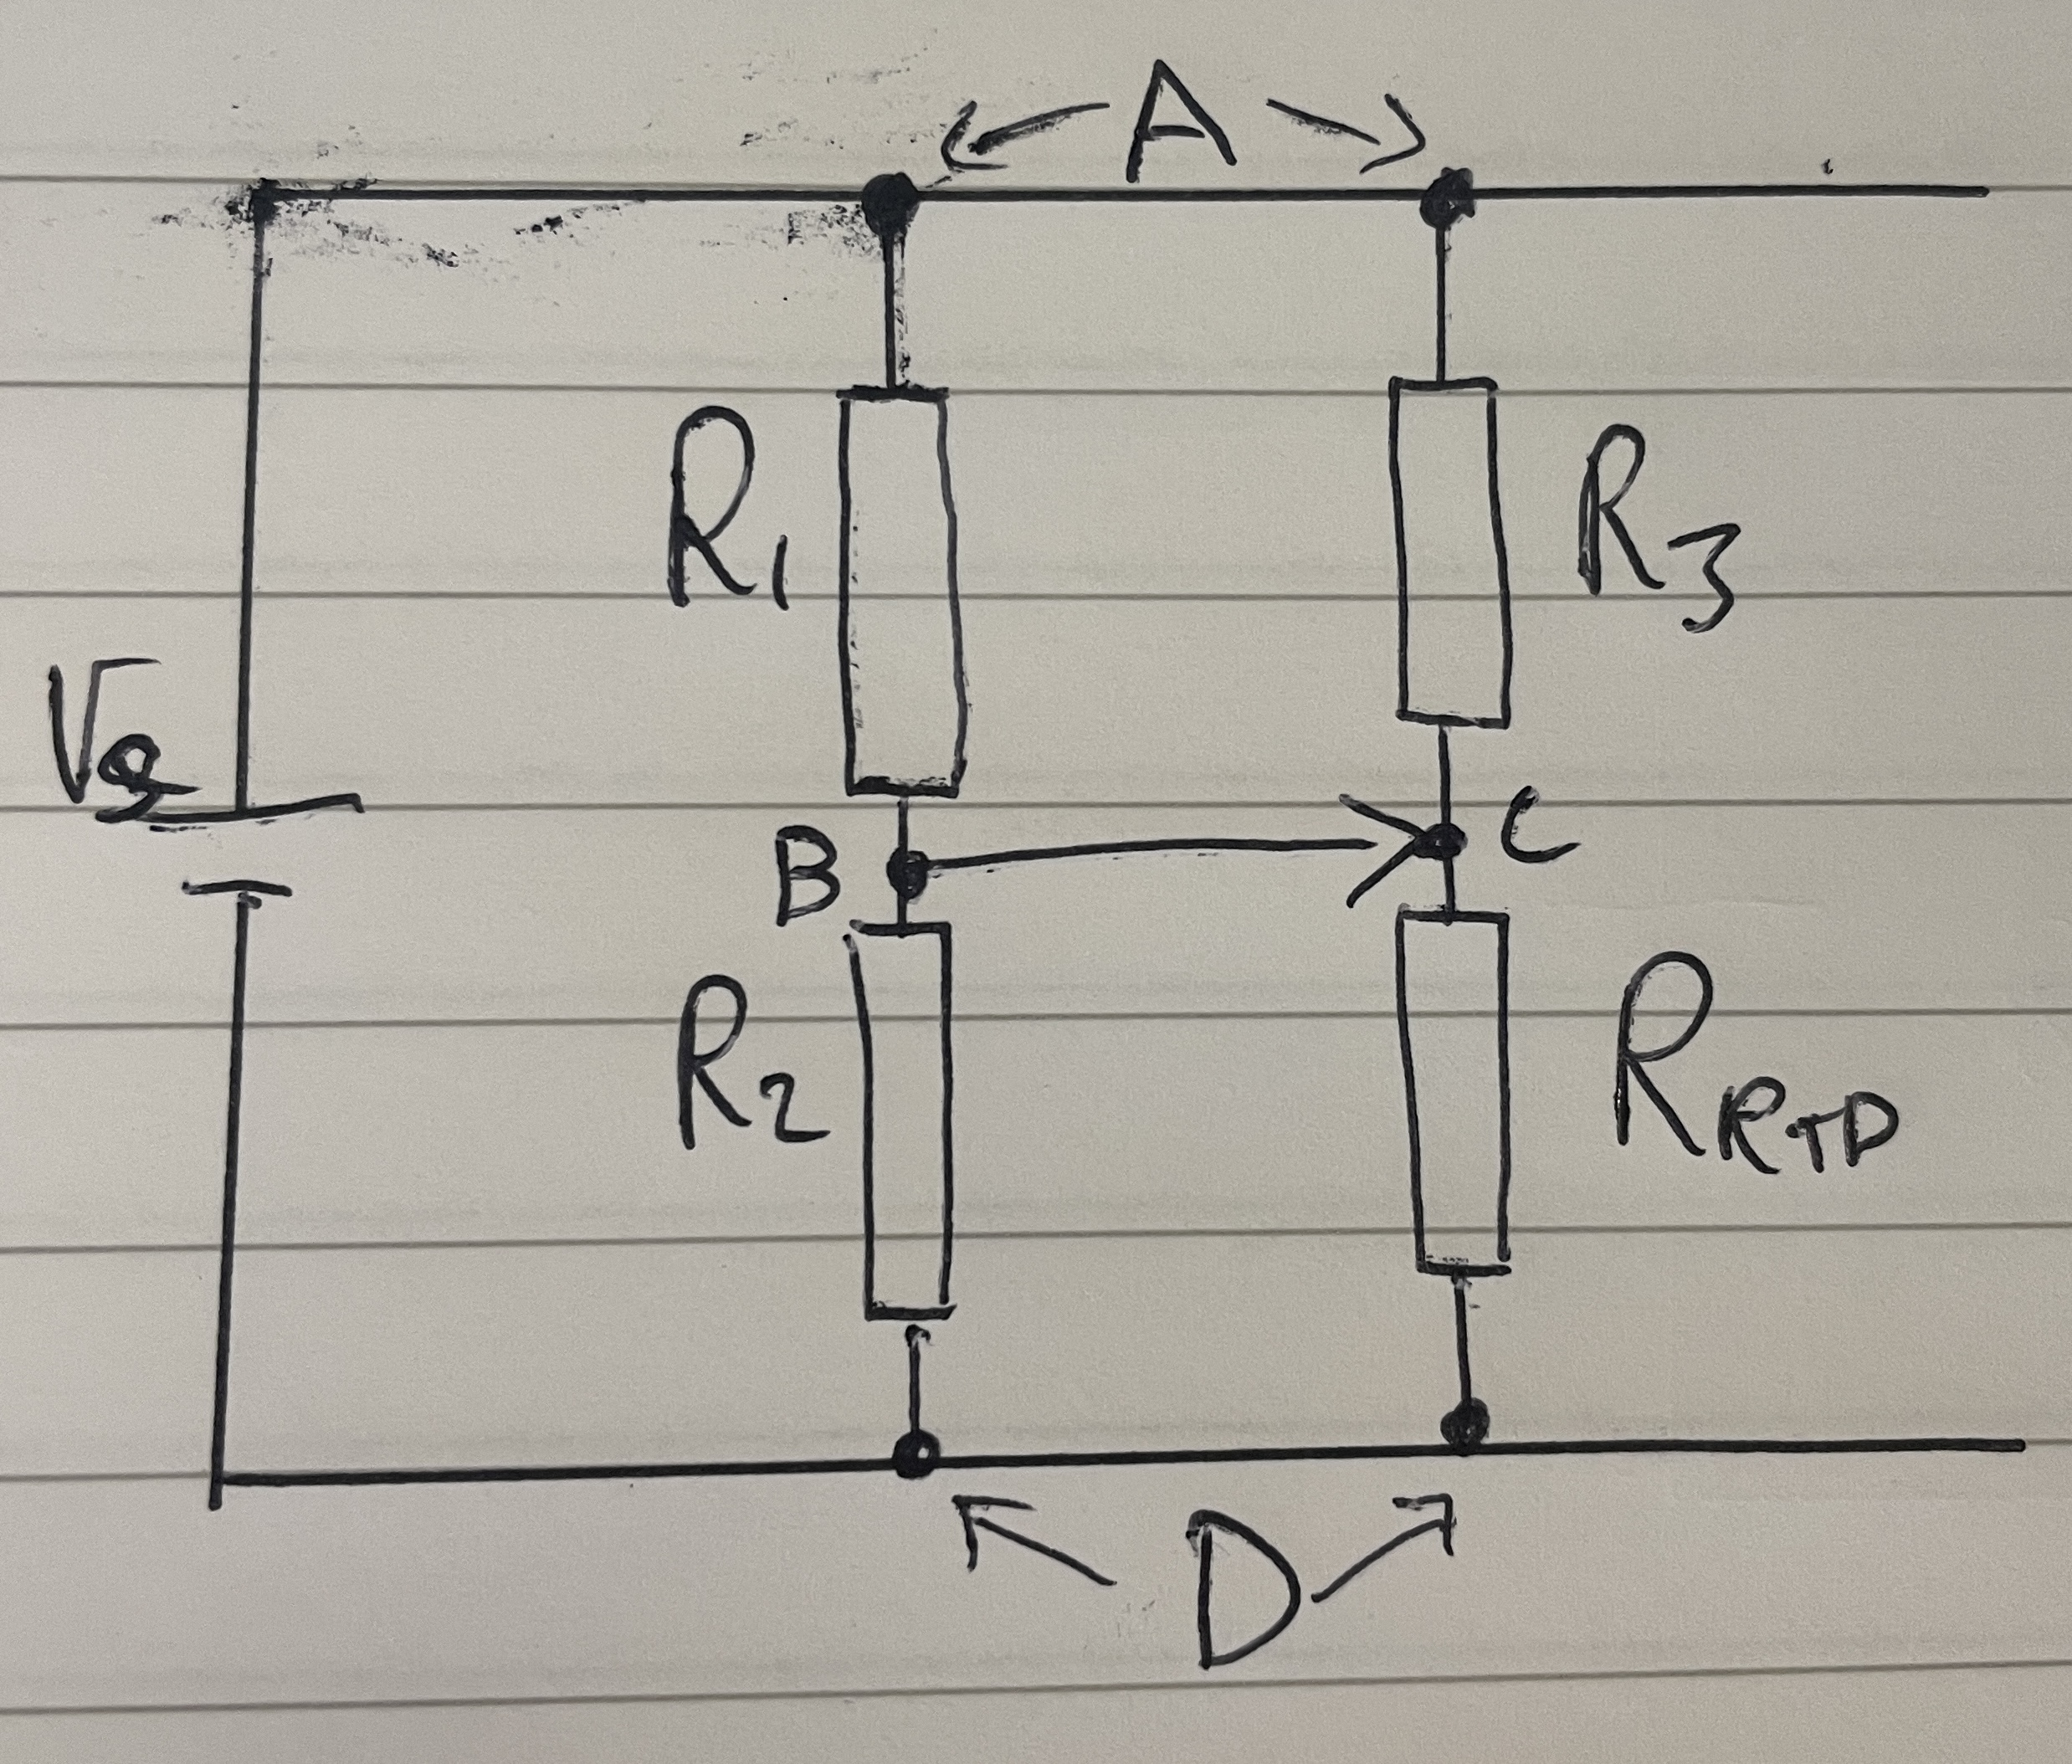
\includegraphics[height = 5cm]{./img/q4a1.jpg}
    \caption{Diagram to show Wheatstone bridge.} 
    \label{fig:q4a1}
\end{figure}
Here:
\begin{align}
    R_1 &= R_2 = R_3 = R\\
    V_C - V_D &= \frac{R_{RTD}}{R+ R_{RTD}}V_s\\
    V_o &= V_C - V_B = \left(V_D + \frac{R_{RTD}}{R+ R_{RTD}}V_s\right) - \left(V_D + \frac{V_s}{2}\right)\\
    V_o &= \left(\frac{R_{RTD}}{R+R_{RTD}} - \frac{1}{2}\right)V_s \label{eq:q4a2}
\end{align}
Take $R$ to have the same value as $R_{RTD}$ at \SI{0}{\celsius} (\SI{1000}{\ohm}), this would balance our bridge at this temperature, i.e. $V_o = 0$. When temperature is above this value, $R_{RTD} = R(1+x)$ where $x$ is increase in resistance due to measurement. We can then look at the voltage of the bridge to find out temperature value:
\begin{align}
    V_o &= \left(\frac{R(1+x)}{R + R(1+x)} - \frac{1}{2}\right)V_s\\
    V_o &= \frac{x}{2(2+x)}V_s
\end{align}
We also know that the temperature is related via \ref{eq:q4a3}. Rearranging \ref{eq:q4a2} and substituting into \ref{eq:q4a3}. 
\begin{align}
    R_{RTD} &= R \left(1+\alpha\left(T - T_0\right)\right) \label{eq:q4a3}\\
    R_{RTD} &= \left(\frac{1}{2} + \frac{V_o}{V_s}\right)\left(R + R_{RTD}\right)\\
    R_{RTD}\left(\frac{1}{2}-\frac{V_o}{V_s}\right) &= R\left(\frac{1}{2}+\frac{V_o}{V_s}\right)\\
    R_{RTD} &= \frac{R\left(\frac{1}{2} + \frac{V_o}{V_s}\right)}{\left(\frac{1}{2}-\frac{V_o}{V_s}\right)}\\
    R_{RTD} &= \frac{R\left(V_s + 2V_o\right)}{V_s - 2V_o}\\
    \frac{R\left(V_s + 2V_o\right)}{V_s - 2V_o} &= R \left(1+\alpha\left(T - T_0\right)\right)\\
    \alpha T &= \frac{\left(V_s + 2V_o\right)}{V_s - 2V_o}-1 \\
    \alpha T &= \frac{V_s + 2V_o}{V_s - 2V_o} - \frac{V_s - 2V_o}{V_s - 2V_o} \\
    T &= \frac{4V_o}{\alpha\left(V_s - 2V_o\right)} \label{eq:q4a4}
\end{align}
\subsection{b}
The metallic resistance thermometer is a good fit for this application as it can measure within the temperature range specified (\SI{0}{\celsius} - \SI{200}{\celsius}). It also has very good linearity. Disadvantages of an RTD include high cost and slow transient response to temperature changes. A thermocouple would not be a good fit as they are typically designed for higher temperature ranges and have a non-linear output. A thermistor could serve as a replacement and have fast transient response but their output is exponential, requiring additional signal processing. 
\subsection{c}
Our uncertainty is coming from two sources here: output voltage $V_o$ and temperature coefficient $\alpha$. Our resistor uncertainties do not contribute to the final uncertainty as the Wheatstone bridge balances any imperfections. Therefore our uncertainty in $T$:
\begin{align}
    \Delta T = \sqrt{\left(\Delta V_o \dfrac{\partial T}{\partial V_o}\right)^2 + \left(\Delta \alpha \dfrac{\partial T}{\partial \alpha}\right)^2} \label{eq:q4c1}
\end{align}
Differentiating:
\begin{align}
    \dfrac{\partial T}{\partial V_o} &= \dfrac{4}{\alpha\left(V_s - 2V_o\right)} + \frac{8V_0}{\alpha\left(V_s -2V_o\right)^2}\\
    \dfrac{\partial T}{\partial V_o} &= \dfrac{4V_s}{\alpha\left(V_s - 2V_o\right)^2}\\
    \dfrac{\partial T}{\partial \alpha} &= \frac{-4V_o}{\alpha^2\left(V_s - 2V_o\right)}
\end{align}
Substituting into \ref{eq:q4c1}:
\begin{align}
    \Delta T = \sqrt{\left(\Delta V_o \dfrac{4V_s}{\alpha\left(V_s - 2V_o\right)^2}\right)^2 + \left(\Delta \alpha \frac{-4V_o}{\alpha^2\left(V_s - 2V_o\right)}\right)^2}  
\end{align}
Dividing by $T$:
\begin{align}
    \dfrac{\Delta T}{T} &= \dfrac{\sqrt{\left(\Delta V_o \dfrac{4V_s}{\alpha\left(V_s - 2V_o\right)^2}\right)^2 + \left(\Delta \alpha \dfrac{-4V_o}{\alpha^2\left(V_s - 2V_o\right)}\right)^2}}{\dfrac{4V_o}{\alpha\left(V_s - 2V_o\right)}}\\
    \dfrac{\Delta T}{T} &= \sqrt{\left(\frac{\alpha\left(V_s - 2V_o\right)}{4V_o}\right)^2} \sqrt{\left(\Delta V_o \dfrac{4V_s}{\alpha\left(V_s - 2V_o\right)^2}\right)^2 + \left(\Delta \alpha \dfrac{-4V_o}{\alpha^2\left(V_s - 2V_o\right)}\right)^2}\\
    \dfrac{\Delta T}{T} &= \sqrt{\left(\Delta V_o \dfrac{4V_s}{\alpha\left(V_s - 2V_o\right)^2}\cdot\frac{\alpha\left(V_s - 2V_o\right)}{4V_o}\right)^2 + \left(\Delta \alpha \dfrac{-4V_o}{\alpha^2\left(V_s - 2V_o\right)}\cdot\frac{\alpha\left(V_s - 2V_o\right)}{4V_o}\right)^2}\\
    \dfrac{\Delta T}{T} &= \sqrt{\left(\dfrac{\Delta V_o}{V_o}\dfrac{V_s}{V_s - 2V_o}\right)^2 + \left(-\dfrac{\Delta \alpha}{\alpha}\right)^2} \label{eq:q4c2}
\end{align}
Rearranging \ref{eq:q4a4} for $V_o$ and substituting into \ref{eq:q4c2}:
\begin{align}
    V_o &= \dfrac{V_s \alpha T}{4+2\alpha T}\\
    \dfrac{\Delta T}{T} &= \sqrt{\left(\dfrac{\Delta V_o}{V_o}\dfrac{V_s}{V_s - 2\dfrac{V_s \alpha T}{4+2\alpha T}}\right)^2 + \left(-\dfrac{\Delta \alpha}{\alpha}\right)^2}\\
    \dfrac{\Delta T}{T} &= \sqrt{\left(\dfrac{\Delta V_o}{V_o}\dfrac{1}{1 - \dfrac{ \alpha T}{2+\alpha T}}\right)^2 + \left(-\dfrac{\Delta \alpha}{\alpha}\right)^2}\\
\end{align}
Substituting the following values:
\begin{gather}
    \dfrac{\Delta V_o}{V_o} = 0.01, \; \dfrac{\Delta \alpha}{\alpha} = 0.001, \; T = \SI{180}{\celsius}, \; \alpha = 0.00375
\end{gather}
\begin{align}
    \dfrac{\Delta T}{T} &= \sqrt{\left(0.01\dfrac{1}{1 - \dfrac{ 0.00375 \times 180}{2+0.00375 \times 180}}\right)^2 + \left(-0.001\right)^2}\\
    \dfrac{\Delta T}{T} &= 0.0134 = 1.34\%
\end{align}
Hence, the uncertainty in the temperature measurement at \SI{180}{\celsius} is:
\begin{align}
    T = 180\pm\SI{2.41}{\celsius} 
\end{align}
\begin{thebibliography}{00}
    \bibitem{b1} Howard Hodson, University of Cambridge, Department of Engineering, Whittle Laboratory "Constant Temperature Anemometers", \url{http://www-g.eng.cam.ac.uk/whittle/current-research/hph/cta-circuit/cta-circuit.html} Accessed 10/05/21 23:05 
    \bibitem{b3} TSI, "TSI Thermal Anemometry Probes", \url{https://www.tsi.com/getmedia/2e3fafd5-8037-40a9-aa38-4fa05a1d3ef3/Hotwire_Catalog_2980465?ext=.pdf} Accessed 11/05/21 00:43
    \bibitem{b2} eFunda Inc, "Hot wire theory", \url{hhttps://www.efunda.com/designstandards/sensors/hot_wires/hot_wires_theory.cfm} Accessed 11/05/21 00:09
\end{thebibliography}
\end{document}